%
%    PhD Thesis
% ~~~~~~~~~~~~~~~~~
%  Master Document
%

\documentclass[twoside,openright,12pt]{book}

% ================================================================================================================================ %

% Main Packages
%***************

% Main
\usepackage[utf8]{inputenc}
\usepackage[UKenglish]{babel}
\usepackage[T1]{fontenc}

% Math
\usepackage{nicefrac}
%\usepackage{xfrac}
\usepackage{amsmath}
\usepackage{amssymb}
\usepackage{mathtools}

% Bibliography
\usepackage[numbers,sort&compress]{natbib}
\bibliographystyle{PhD}                   % Custom citation style
\usepackage{doi}                          % Makes DOIs clickable

% Layout
\usepackage[a4paper]{geometry}            % Page geometry
\usepackage{emptypage}                    % Prevents page numbers on empty pages
\usepackage{setspace}                     % Line spacing
\usepackage{titlesec}                     % Alternative section titles
\usepackage{fancyhdr}                     % Changing headers and footers
\usepackage{tocloft}                      % For modifying the Table of Contents
\usepackage{appendix}                     % Added functionality for appendices
\usepackage{enumerate}                    % Allows for Roman numbered lists
\usepackage{float}                        % Floating of figures and tables

% Fonts
\usepackage[scaled]{raleway}              % Raleway font for sans-serif text
\usepackage[scaled]{sourcecodepro}        % Source Code Pro font for typewriter text
\usepackage{textcomp}                     % Adds additional text symbols
\usepackage{tgtermes}                     % TEX Gyre Termes font

% Content
\usepackage{pdfpages}                     % Include PDF files
\usepackage{datetime}                     % Used for the last page timestamp
\usepackage{todonotes}                    % Add Todo notes

% Tables
\usepackage{array}                        % Used for centred p elements
\usepackage{tabularx}                     % Allows full width tables
\usepackage{colortbl}                     % Allows table colouring
\usepackage{dcolumn}                      % Special decimal cells

% ================================================================================================================================ %

% Document Layout
%*****************

\geometry{twoside,left=25mm,right=25mm,top=30mm,bottom=30mm}
\AtBeginDocument{\parskip=0pt plus 2.5pt\relax\setstretch{1.1}}

% Fix section numbering bug in Titlesec
\usepackage{etoolbox}
\makeatletter
\patchcmd{\ttlh@hang}{\parindent\z@}{\parindent\z@\leavevmode}{}{}
\patchcmd{\ttlh@hang}{\noindent}{}{}{}
\makeatother

% Stretches text to fix underfull or overfull errors
\usepackage[activate=true,final,stretch=10,shrink=10]{microtype}

% Silence underfull errors for bibliography
\apptocmd{\sloppy}{\hbadness 10000\relax}{}{}

% Colours
\usepackage{color}
\definecolor{chapter} {gray}{0.60}
\definecolor{appendix}{gray}{0.50}
\definecolor{capcol}  {gray}{0.25}
\definecolor{tblhead} {rgb}{0.929,0.792,0.467}
\definecolor{tblco}   {rgb}{0.970,0.970,1.000}
\definecolor{tblce}   {rgb}{0.930,0.930,1.000}
\definecolor{tblunit} {rgb}{0.929,0.863,0.698}
\definecolor{tblfoot} {gray}{0.90}
\definecolor{ttcol}   {rgb}{0.333,0.039,0.098}
\definecolor{emcol}   {rgb}{0.333,0.039,0.098}
\definecolor{d-blue}  {rgb}{0.000,0.200,0.741}
\definecolor{d-red}   {rgb}{0.850,0.125,0.000}
\definecolor{d-green} {rgb}{0.231,0.333,0.094}
\definecolor{m-blue}  {rgb}{0.000,0.447,0.741}
\definecolor{m-red}   {rgb}{0.850,0.325,0.098}
\definecolor{m-yellow}{rgb}{0.929,0.694,0.125}
\definecolor{m-purple}{rgb}{0.494,0.184,0.556}
\definecolor{m-green} {rgb}{0.466,0.674,0.188}
\definecolor{m-cyan}  {rgb}{0.301,0.745,0.933}
\definecolor{m-brown} {rgb}{0.635,0.078,0.184}

% MATLAB Colours
%================
% Blue      0.000  0.447  0.741      0   114   189    0072bdff
% Red       0.850  0.325  0.098    217    83    25    d95319ff
% Orange    0.929  0.694  0.125    237   177    32    edb120ff
% Purple    0.494  0.184  0.556    126    47   142    7e2f8eff
% Green     0.466  0.674  0.188    119   172    48    77ac30ff
% Cyan      0.301  0.745  0.933     77   190   238    4dbeeeff
% Brown     0.635  0.078  0.184    162    20    47    a2142fff

% Links
\usepackage{bookmark}
\usepackage[verbose,hyperpageref]{backref}
\usepackage{hyperref}
% \usepackage{url}
\hypersetup{colorlinks=true, citecolor=d-blue, urlcolor=d-blue, linkcolor=m-brown}
\urlstyle{same}
\renewcommand*{\backrefalt}[4]{\ifcase #1 No citations.\or Cited on page #2.\else Cited on pages #2.\fi}

% Tables
\newcommand{\texthh}[1]{\textsc{#1}}
\newcommand{\texthu}[1]{\small\textsc{#1}}
\newcommand{\textun}[1]{\small[\texttt{#1}]}
\renewcommand{\arraystretch}{1.16}
\newcolumntype{d}[1]{D{.}{.}{#1}}
\newcolumntype{L}[1]{>{\raggedright\arraybackslash}p{#1}}
\newcolumntype{C}[1]{>{\centering\arraybackslash}p{#1}}
\newcolumntype{R}[1]{>{\raggedleft\arraybackslash}p{#1}}

% Figures
%\floatstyle{boxed}
%\restylefloat{figure}

% Captions
\usepackage[font={color=capcol}]{caption}
\captionsetup[table]{labelfont=sc,skip=8pt}
\captionsetup[figure]{labelfont=sc}

% Text
\renewcommand{\rmdefault}{ptm} % Times
% \renewcommand{\sfdefault}{sb}
% \renewcommand{\ttdefault}{sourcecodepro}
\renewcommand{\texttt}[1]{\textcolor{ttcol}{\small\ttfamily #1}}
\renewcommand{\emph}[1]{\textcolor{emcol}{\slshape #1}}

% TOC
%% Content
\renewcommand\cftpartfont{\sffamily\large}
\renewcommand\cftpartpagefont{\mdseries}
\renewcommand\cftchapfont{\mdseries}
\renewcommand\cftchappagefont{\mdseries}
\renewcommand\cfttoctitlefont{\huge\sffamily}

%% List of Figures
\renewcommand\cftloftitlefont{\huge\sffamily}
\renewcommand\cftfigindent{0pt}
\renewcommand\cftfignumwidth{65pt}
\renewcommand\cftfigpresnum{Figure~}

%% List of Tables
\renewcommand\cftlottitlefont{\huge\sffamily}
\renewcommand\cfttabindent{0pt}
\renewcommand\cfttabnumwidth{65pt}
\renewcommand\cfttabpresnum{Table~}

% ================================================================================================================================ %

% Custom Commands
%*****************

% Text
\newcommand{\eq}[1]{Eq. \ref{#1}}
\newcommand{\fig}[1]{Fig. \ref{#1}}
\newcommand{\tbl}[1]{Table \ref{#1}}
\newcommand{\ts}[1]{\textsuperscript{#1}}
\newcommand{\dash}{\textendash~}
\newcommand{\celsius}{\,^{\circ}\mathrm{C}}
\newcommand{\etal}{\textit{et~al.}}

% Math Commands
\newcommand{\unit}[1]{\,\mathrm{#1}}
\newcommand{\funit}[2]{\,\nicefrac{\mathrm{#1}}{\mathrm{#2}}}
\newcommand{\mexp}[1]{\mathrm{e}^{#1}}
\newcommand{\nexp}[1]{\times 10^{#1}}
\newcommand{\deriv}{\mathrm{d}}
%\newcommand{\ln}{\mathrm{ln}}

% Values
\newcommand{\emitN}[0]{\epsilon_{\mathrm{N}}}
\newcommand{\emitg}[0]{\epsilon_{\mathrm{g}}}
\newcommand{\gammar}[0]{\gamma_{\mathrm{r}}}
\newcommand{\betar}[0]{\beta_{\mathrm{r}}}

% Hyphenation
\hyphenation{wave-length}
\hyphenation{Swit-zer-land}
\hyphenation{de-fo-cus-ing}
\hyphenation{de-cel-e-rat-ing}

% ================================================================================================================================ %

% Page Layout
%*************

% Plain Page Numbering
\fancypagestyle{plain}{
    \fancyhf{}
    \fancyfoot[LE,RO]{\thepage}
    \renewcommand{\headrulewidth}{0pt}
}

% Header style for numbered chapters
\newcommand{\defaulthead}{
    \fancyhead[LE]{\nouppercase{\scshape\leftmark}}
    \fancyhead[RO]{\nouppercase{\scshape\rightmark}}
}

% Custom heading for unnumbered chapters
\newcommand{\simplehead}[1]{
    \fancyhead[LE]{\nouppercase{\scshape #1}}
    \fancyhead[RO]{\nouppercase{\scshape #1}}
}

\pagestyle{fancy}

% Page Header
\renewcommand{\chaptermark}[1]{\markboth{\thechapter.\ #1}{}}
\renewcommand{\sectionmark}[1]{\markright{\thesection\ #1}{}}
\renewcommand{\headrulewidth}{0.5pt}
\renewcommand{\footrulewidth}{0pt}

\fancyhf{}
\defaulthead
\headheight 15pt
\fancyfoot[LE,RO]{\thepage}

% Parts
\titleformat{\part}[block]{}{}{}{\centering\fontsize{40}{50}\sffamily\scshape}

% Numbered Chapters
\titlespacing*{\chapter}{0mm}{10mm}{20mm}
\titleformat{\chapter}[hang]{\fontsize{60}{70}\sffamily}{\textcolor{chapter}\thechapter}{8mm}{\Huge\sffamily}

% Sections
\setcounter{secnumdepth}{3}
\setcounter{tocdepth}{3}
\titleformat{\section}{\Large\sffamily\mdseries}{\thesection}{2mm}{}
\titleformat{\subsection}{\large\sffamily\mdseries}{\thesubsection}{2mm}{}
\titleformat{\subsubsection}{\normalsize\sffamily\mdseries}{\thesubsubsection}{2mm}{}

% ================================================================================================================================ %

% Main Document
%***************

\begin{document}

% Front Matters

\frontmatter
    \begin{titlepage}
    \begin{center}
        \vspace*{10mm}
        \huge{}
        Preliminary Title:\\
        Plasma Wakefield Acceleration\\
        \vspace{20mm}
        \large
        \textbf{Veronica K. Berglyd Olsen}\\
        Department of Physics\\
        University of Oslo\\
        Norway\\
        \vfill
        
\includegraphics[width=0.35\textwidth]{images/UiOLogo.pdf}\\
        \vspace{20mm}
        Dissertation Presented for the Degree of\\
        Philosophiae Dpctor (PhD) in Physics\\
        \vspace{10mm}
        \large{July 2017}
    \end{center}
\end{titlepage}


    \cleardoublepage
    \pdfbookmark{Abstract}{Abstract}
    \chapter*{Abstract}
Abstract


    \cleardoublepage
    \pdfbookmark{Acknowledgements}{Acknowledgements}
    \chapter*{Acknowledgements}
Acknowledgements


    \tocloftpagestyle{plain}
    \cleardoublepage
    \pdfbookmark{\contentsname}{Contents}
    \microtypesetup{protrusion=false}
    \tableofcontents
    \vfill\pagebreak
    \pdfbookmark{\listfigurename}{List of Figures}
    \backrefsetup{disable}
    \listoffigures
    \backrefsetup{enable}
    \vfill\pagebreak
    \pdfbookmark{\listtablename}{List of Tables}
    \backrefsetup{disable}
    \listoftables
    \backrefsetup{enable}
    \microtypesetup{protrusion=true}
    \cleardoublepage

% Main Matters

\pagestyle{fancy}

\mainmatter
    \phantomsection
    \addcontentsline{toc}{chapter}{Preface}
    \chapter*{Preface}

The work presented in this thesis is published in four papers:

\begin{enumerate}[I]
    \item Loading of a Plasma-Wakefield Accelerator Section Driven by a Self-Modulated Proton Bunch, \emph{Proceedings of IPAC 2015} \cite{berglyd_olsen:2015}
    \item Loading of Wakefields in a Plasma Accelerator Section Driven by a Self-Modulated Proton Beam, \emph{Proceedings of NAPAC 2016} \cite{berglyd_olsen:2016}
    \item Data Acquisition and Controls Integration of the AWAKE Experiment at CERN, \emph{Proceedings of IPAC 2017} \cite{berglyd_olsen:2017}
    \item Emittance Preservation of an Electron Beam in a Loaded Quasi-Linear Plasma Wakefield, \emph{Physical Review Accelerators and Beams} \cite{berglyd_olsen:2017-1}
\end{enumerate}

\noindent The papers are included in this thesis in the \hyperref[A:Pub]{Publications} section.

\section*{Notation}

\begin{table}[hbt]
    \centering
    \caption{Overview of notation used in this thesis.}
    \label{T:Notes}
    \begin{tabular}{p{0.10\linewidth} p{0.78\linewidth}}
        \hline
        \textbf{Notation}           & \textbf{Description} \\
        \hline
        $n_{0}$                     & The average or initial plasma density \\
        $n_{pe}$                    & The density of plasma electrons \\
        $n_{b}$                     & The density of a general particle beam \\
        $n_{eb}$, $n_{pb}$          & The density of an electron or a proton beam in particular \\
        % \hline
        $\sigma_{r}$                & The width of a Gaussian beam when it is assumed to be round \\
        $\sigma_{x}$, $\sigma_{y}$  & The transverse size of a Gaussian beam when it may not be
                                      round, or the value applies to only one plane. \\
        % \hline
        $\alpha$, $\beta$, $\gamma$ & The Twiss parameters, also known as the Courant-Snyder
                                      parameters \cite{courant:1958}. \\
        $\betar$, $\gammar$         & Relativistic factors* \\
        \hline
    \end{tabular}
\end{table}

\paragraph{*}
These are indexed with \emph{r} in this thesis to separate them from the Twiss parameters.

\vfill
    %
%  Introduction
% ==============
%

\chapter{Introduction}
\label{Ch:Intro}

Text

% ================================================================================================ %
\section{Plasma Wakefield Acceleration}
\label{Int:PWFA}

Intro to plasma wakefield goes here

% ================================================================================================ %
\section{Proton Driven Plasma Wakefield Acceleration}
\label{Int:PDPWFA}

Further details on proton driven plasma wakefield goes here.

% ================================================================================================ %
\section{The Self-modulation Instability}
\label{Int:SMI}

Stuff about SMI goes here

% ================================================================================================ %
\section{Numerical Simulations of PWFA}
\label{Int:Sim}

Stuff about Osiris and and all that jazz.

Reference to PIC appendix.

% ================================================================================================ %

    %
%  Wakefield Acceleration
% ========================
%

\chapter{Wakefield Acceleration, an Overview}
\label{Ch:WFA}

Text

% ==================================================================================================================== %
\section{Evolution of the Concept}
\label{WFA:History}

Text

% ==================================================================================================================== %
\section{The Advanced Wakefield Experiment (AWAKE)}
\label{WFA:AWAKE}

Text

% ==================================================================================================================== %
\subsection{AWAKE Run 1}
\label{WFA:AWAKE:R1}

Text

% ==================================================================================================================== %
\subsection{AWAKE Run 2}
\label{WFA:AWAKE:R2}

Text

% ==================================================================================================================== %
\section{The Self-modulation Instability}
\label{WFA:SMI}

Text

% ==================================================================================================================== %
\section{Beam Loading}
\label{WFA:BLoad}

Text

% ==================================================================================================================== %

    %
%  Tools
% =======
%

\chapter{AWAKE Data Acquisition}
\label{Ch:DAQ}


% =============================================================================================== %
\section{Data Acquisition Classes for FESA}
\label{Tools:FESA}

Some text.

% =============================================================================================== %

    %
%  Simulations
% =============
%

\chapter{Simulation Method}
\label{Ch:SimS}

The work presented in this thesis has been performed using simulations with two particle-in-cell (PIC) codes:
OSIRIS~\cite{fonseca:2002} and QuickPIC~\cite{an:2013, huang:2006}.
OSIRIS is a proprietary full PIC code available in 1, 2 and 3 dimensions, with a choice between Cartesian and cylindrical coordinates.
QuickPIC is a quasi-static 3D PIC code, that is available in an open source version~\cite{add:quickpic:web}.
In the simulations presented here, both OSIRIS and the open source version of QuickPIC has been used.
For a more detailed description on PIC codes, see Appendix~\ref{Apx:PIC}.

Although PIC codes use macro particles -- that is simulated particles represent more than one physical beam or plasma particle -- these codes require a lot of CPU power.
This is especially true when running 3D simulations.
The preliminary studies presented in Publications~\ref{Pub:IPAC15} and~\ref{Pub:NAPAC16} were done using OSIRIS with 2D cylindrical coordinates.
The main study, Publication~\ref{Pub:BL17}, was done using QuickPIC in 3D Cartesian coordinates.
In order to perform the detailed parameter scans needed for these studies, the drive beam and accelerating structure had to be scaled down into a more manageable size than simulating the full SPS proton bunch would require.
The full SPS proton bunch is orders of magnitude larger than both the electron bunch and the plasma wavelength, as can be seen in Table~\ref{T:AWAKERuns}.
This chapter will outline the simulation environment chosen for these studies, and the reasons behind these.

% ================================================================================================================================ %
\section{Simulating the Drive Bunch}
\label{Sim:PBeam}

An initial set of simulations were run to study the evolution of the self-modulation instability in the SPS proton bunch.
These simulations assumed the plasma was ionised at the centre of the bunch (see Section~\ref{Int:DBeam:SMI}), so only the back half of it was actually simulated.
The beam profile function used took the form:
\begin{equation}
    f(\xi,r) = \frac{A_{q}}{2} \left[1 + \cos\left(\xi\frac{\pi}{L}\right)\right] \exp\left(-\frac{r^{2}}{2\sigma_{r}^{2}}\right), \label{EQ:SPS-Profile}
\end{equation}
where $L = 2.5\sigma_{z,pb} = 30\unit{cm}$ is the length of half an SPS proton bunch, $R$ is the radius of the simulation box, and $A_{q}$ is a charge scaling factor such that the total charge of the half bunch matches the charge outlined in Table~\ref{T:AWAKERuns}.
The charge of the simulated proton bunch in cylindrical coordinates is given by:
\begin{equation}
    Q_{pb} = 2\pi \iint f(\xi,r) \;r \deriv r \deriv \xi, \label{EQ:SPS-Charge}
\end{equation}
A half period cosine function for the longitudinal density profile is more convenient for simulations than a Gaussian shape as the cosine goes to zero at a finite length~\cite{lotov:2010}.
Radially, the bunch is still Gaussian, and requires a cut-off to be added to prevent OSIRIS from generating macro particles with small weights.
The CPU cost is proportional to the number of simulation particles, regardless of weight.
An example of the SPS proton bunch before and after self-modulated has occurred, as simulated in OSIRIS 3.0, can be seen in Figure~\ref{Fig:Sim:SMI}.

\begin{figure}[hbt]
    \centering
    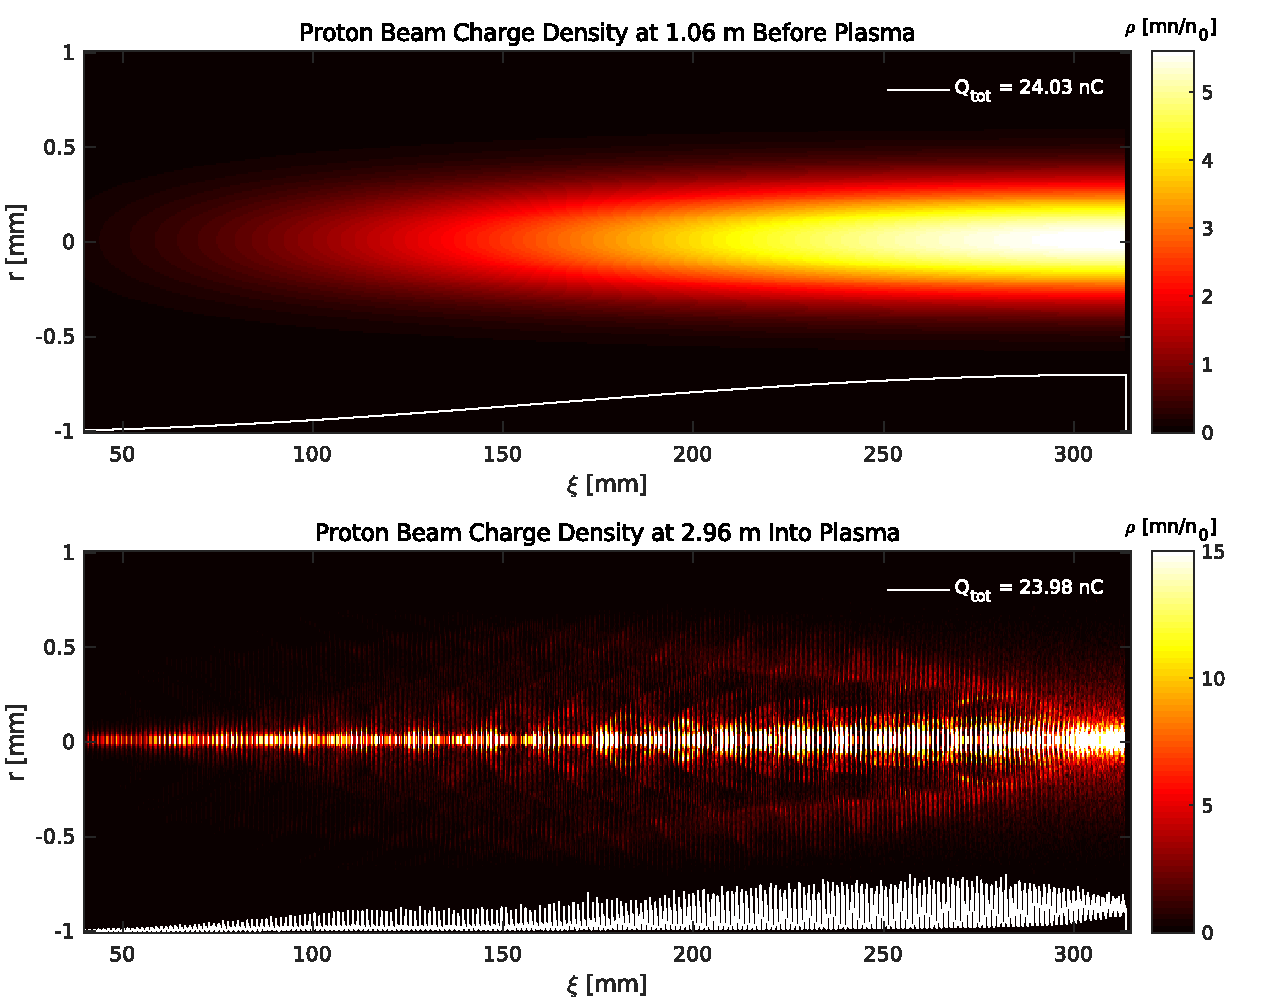
\includegraphics[width=1.0\linewidth]{figures/PBSelfModulationBefAft}
    \caption{\label{Fig:Sim:SMI}
        \textbf{Top:} An example of a simulation of half SPS proton bunch before reaching plasma.
        \textbf{Bottom:} The same bunch after having undergone self-modulation in about $3\unit{m}$ of plasma.
        The halo of protons ejected from the defocusing regions can be clearly seen, leaving a core of micro bunches on the beam axis.
    }
\end{figure}

% ================================================================================================================================ %

\subsection{With a Pre-Modulated Beam}
\label{Sim:PBPreMod}

The half SPS proton bunch is about $30\unit{cm}$ long, or $238\lambda_{pe}$, which requires a large number of grid cells to resolve.
In order to make the simulations more manageable in size for the beam loading studies, we decided to move to a sample proton bunch of 26 micro bunches -- an order of magnitude smaller than the previous case.

These simulations were all done using OSIRIS 3.0.
With this version it is necessary for the beams to drift in vacuum for a short distance for the electro-magnetic fields to develop properly, as they are initialised at zero (see further discussion in Section~\ref{PIC:Full}).
Since the evolution of the self-modulation instability was not of primary interest at this stage, we chose to modify the bunch profile to emulate a section of the modulated bunch.
We refer to this as \textit{pre-modulation}.
This was done by shortening the period of the density envelope cosine function from Equation~\ref{EQ:SPS-Profile} to match that of the plasma wavelength.
\begin{equation}
    f(\xi,r) = A\sqrt{2} \left[\frac{1}{2\sqrt{2}}
             + \cos\left(k_{pe}\xi - \mu\right)\right] \exp\left(-\frac{r^{2}}{2\sigma_{r}^{2}}\right), \label{EQ:PB-PreMod}
\end{equation}
where $\mu$ is the position of the first micro bunch, and $k_{pe}$ is the plasma wave number~\cite{berglyd_olsen:2015}.
The offset of the cosine function is chosen such that the width of the micro bunch matches the width of a bunch in the simulations done with a full SPS bunch, and there is a gap between the bunches that approximates the gaps we see between micro bunches in the simulated self-modulated case.
Since OSIRIS ignores profile densities with negative values, the profile is automatically clipped at $0$, requiring no further manipulation of the profile function to remove negative values.

Again, cosines are preferred over a series of Gaussian bunch profiles, although this time because the cosine is periodic, and because OSIRIS' mathematical functions cannot be longer than 256 characters.

Generating an equidistant bunch train in this manner causes the head of the second bunch to be partially defocused causing a decay of the micro bunches by the wakefield of the first bunch.
This effect was not directly compensated for in Publication~\ref{Pub:IPAC15}.
This can be avoided by increasing the separation between the first and second bunch from $2\pi c/\omega_p$ to $(2\pi+\pi/4) c/\omega_p$~\cite{lotov:2018}.

The charge of the proton micro bunches were matched to that of a micro bunch generated by the self-modulation instability in the initial simulations.
The charge density decreases towards the back end of the self-modulated bunch (see Figure~\ref{Fig:Sim:SMI}), so for the pre-modulated set-up the densities of the micro bunches were fixed to a charge for the region were the injection of an electron bunch is reasonable -- that is, around 100 plasma wavelengths behind the laser pulse.
For the pre-modulated simulations, this charge was set to $100\unit{pC}$ such that the total charge of the sample proton beam was $2.6\unit{nC}$.
This corresponds to a peak current of $135\unit{A}$.
The electron witness bunch was injected between bunch 20 and 21.

\begin{figure}[hbt]
    \centering
    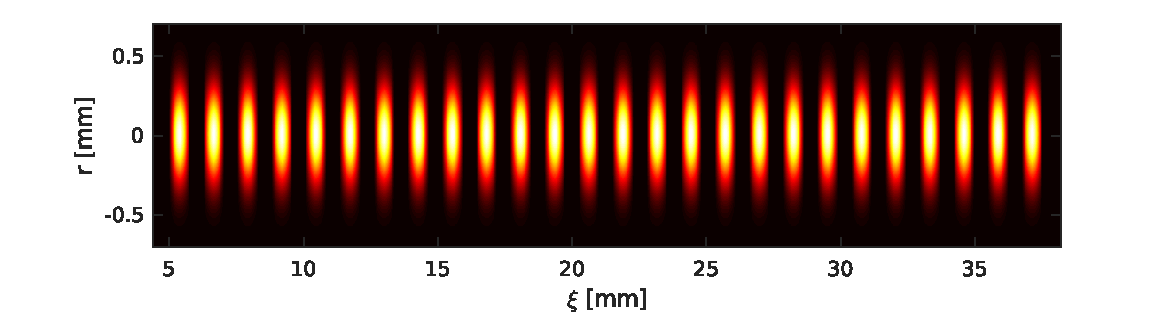
\includegraphics[width=0.9375\linewidth,trim={0mm 0mm 0mm 0mm},clip]{figures/PBPreMod}
    \caption{\label{Fig:PBPreMod}
        An example of a pre-modulated beam of 26 micro-bunches modulated at the plasma wavelength.
        This simulation set-up was used for Publication~\ref{Pub:IPAC15}.
        The density function (see Equation~\ref{EQ:PB-PreMod}) is tuned to match the earlier self-modulation simulations shown in Figure~\ref{Fig:Sim:SMI}.
    }
\end{figure}

% ================================================================================================================================ %

\subsection{With a Single Drive Bunch}
\label{Sim:PBSingle}

Further approximations needed to be made to decrease the scale of the problem in order to study the beam loading and evolution of the electron witness beam more directly.
Even the pre-modulated proton beam is somewhat costly to simulate -- both because it still requires a multiple plasma-wavelength simulation box length, and because a large number of simulated particles are needed to populate the beam profile.
These proved to be a challenge when doing larger parameter scans as the CPU cost would rise to levels beyond available resources.
While additional resources could potentially have been requested, we considered the option to exclude the evolution of the proton bunch entirely from our studies and instead assume the region where the electron bunch was injected to have the properties laid out in the AWAKE status reports~\cite{awake_collaboration:2016}.

In these single bunch studies we therefore approximated the proton drive beam ahead of the witness bunch injection region as a single, ideal proton drive bunch generating the expected wakefields.
To reproduce these conditions, we used a Gaussian bunch of $1.46\nexp{10}$ protons corresponding to $2.34\unit{nC}$, a length $\sigma_{z} = 40\unit{\mu m}$ corresponding to $7\unit{kA}$, and a transverse size $\sigma_{x,y}=200\unit{\mu m}$~\cite{berglyd_olsen:2018}.
To prevent the proton bunch from evolving at the time scale we were interested in for these studies -- up too a $100\unit{m}$ of plasma -- we also increased the mass of the bunch protons by a factor of $1\nexp{6}$.
This effectively froze the wakefields both longitudinally and transversely, and the only evolution of the wakefields was that which was caused by the electron witness bunch itself.

\begin{figure}[hbt]
    \centering
    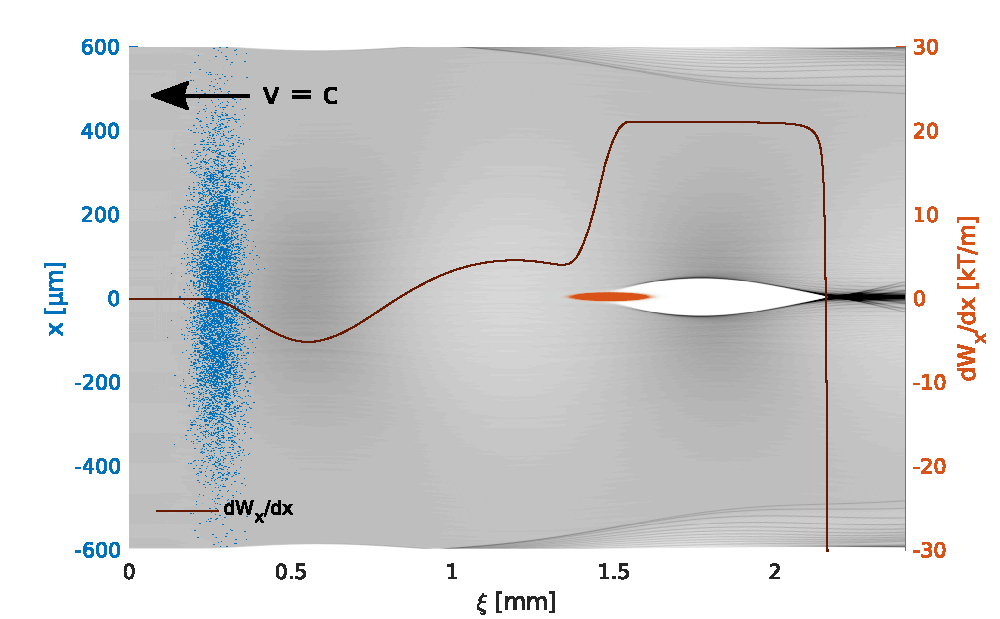
\includegraphics[width=0.8125\linewidth,trim={0mm 0mm 0mm 0mm},clip]{figures/SingleBunchPB}
    \caption{\label{Fig:PBSingle}
        An example of the simulation set-up used for Publication~\ref{Pub:BL17}.
        These simulations used a a single, rigid proton bunch in blue, with a charge large enough to generate a wakefield equivalent to what we expect from the SPS proton bunch in AWAKE Run~2.
        The electron witness bunch is shown in red, and the plasma density is shown in grey where the white region is the plasma bubble void of plasma electrons.
        Note that in the QuickPIC simulations the simulation box travels towards the left, towards $\xi = 0$.
    }
\end{figure}

Figure~\ref{Fig:PBSingle} shows the simulation setup that was used for Publication~\ref{Pub:BL17}, and shows both the proton bunch in blue, and the electron bunch in red.
The plasma can be seen as a grey shaded area where the regions void of plasma electrons can be seen in white.
This is mainly the bubble driven by the high charge density electron bunch, but also as ripples on the edge of the plasma channel.
The density perturbation and longitudinal wakefield generated by the proton bunch falls in the quasi-linear regime, as illustrated in Figures~\ref{Fig:BPI:Regime} and~\ref{Fig:BPI:Density}.

% ================================================================================================================================ %
\section{Simulating the Witness Bunch}
\label{Sim:EBeam}

Simulating the witness bunch is generally straight forward as we have only considered a single bunch with a Gaussian shape both longitudinally and transversely.
However, there are a few things to keep in mind when setting up the beam profile.

% ================================================================================================================================ %
\subsection{Witness Bunch Size and Resolution}
\label{Sim:EBeam:SizeRes}

For the early simulations, a transverse size of $\sigma_{x,y}=105\unit{\mu m}$ was used, see Table~\ref{T:AWAKERuns}.
For later simulations, when the bunch transverse size was matched to its emittance and the plasma density (see Section~\ref{Int:BPI:Match}), much narrower bunches were used -- on the order of a few micrometres.
The proton drive bunch size is tied to the plasma skin depth (see Section~\ref{Int:DBeam:SMI}), which is $200\unit{\mu m}$.
This, naturally, poses a resolution challenge when very narrow electron bunches need to be resolved, while at the same time, the simulation box needs to also be able to contain the proton drive bunch.

For the simulations with a pre-modulated proton beam, used for Publication~\ref{Pub:IPAC15}, the simulation box had a radius of $2.12\unit{mm}$ with $425$ grid cells, resulting in a resolution of $5\unit{\mu m}$.
This is more than sufficient to resolve and contain both the proton beam and the electron bunch, with a small buffer for the plasma (see Section~\ref{Sim:Plasma}).
For the single drive bunch studies, Publications~\ref{Pub:NAPAC16} and~\ref{Pub:BL17}, the transverse grid resolution had to be increased.
In most cases we tried to resolve the witness bunch with at least $5$ grid cells per $\sigma_{x,y}$, although this was in some instances increased.
It was also important to keep an eye on the distribution of macro particles on the simulation grid.
This was especially important for the OSIRIS 3.0 based simulations, as OSIRIS creates macro particles of varying charge, with a fixed number of particles per cell defined by input parameters.
Since most OSIRIS simulations were run with a 2D cylindrical geometry, a $1/r$ factor enters into the electromagnetic field equations.
This results in numerical noise when $r \to 0$, which in return affects the evolution of the bunch itself.
A sample of the 2D cylindrical simulations were re-run with 3D Cartesian coordinates in order to check that the results were not dominated by this noise.
While the 3D simulations were much smoother along the beam axis, the actual results did not seem to differ to any significant degree.

QuickPIC uses 3D Cartesian coordinates, and thus, as OSIRIS 3D, does not have the $1/r$ problem.
In addition, QuickPIC has a fixed charge per bunch macro particle, and instead varies the number of these per grid cell to create a charge distribution.
A convergence scan of resolution dependency was performed for Publication~\ref{Pub:BL17} to check that the results did not depend on resolution within the range we used for this study. The convergence scan is described in Section~\ref{SimA:Converge}.
QuickPIC defines resolution in exponents of $2$, and thus are locked to a set of values that rapidly increase for each step.
The simulations used for Publication~\ref{Pub:BL17} were done with transverse grids of $2^{9}$ and $2^{10}$ ($512 \times 512$ and $1024 \times 1024$) cells, resolving a box size of $1.2\unit{mm}$ square.
In the former case, the grid cell size was thus as large as $2\unit{\mu m}$ for the former case, and $1\unit{\mu m}$ for the latter.
This did, however, not appear to have any significant impact on the results.

Further details on how QuickPIC and OSIRIS handle bunch particles is covered in Appendix~\ref{Apx:PIC}.

% ================================================================================================================================ %
\subsection{Witness Bunch Transverse Evolution}
\label{Sim:EBeam:TEvol}

In OSIRIS 3.0, the electromagnetic fields are initialised at zero.
It is therefore necessary to let the bunches drift a short distance before they enter the plasma region in order for the fields to develop.
Due to this initial drift stage, it was technically challenging to inject an electron witness bunch while strictly controlling parameters like emittance, energy spread and transverse size during the drift phase.
These parameters undergo evolution during this initial drift.
It is, however, possible to prevent the beam from evolving by slowly ramping up the beam charge or the beam energy.
During these ramping stages the macro particles are prevented from transverse evolution.

For the early studies, and for Publication~\ref{Pub:IPAC15}, only beam loading and acceleration were considered.
For Publications~\ref{Pub:NAPAC16} and \ref{Pub:BL17} it was, however, necessary to control the witness bunch emittance.
While QuickPIC has input parameters defining beam emittance in each direction, OSIRIS 3.0 does not.
OSIRIS 3.0 does let one define spatial and momentum distributions independently (see Appendix~\ref{Apx:PIC}).
However, as correlation between $\sigma_{p_{i}}$ and $\sigma_{i}$, for dimension $i$, cannot be controlled, the beam can only be initialised at waist (Twiss parameter $\alpha = 0$, see Appendix~\ref{Apx:DA}).

For the OSIRIS simulations, the ramping parameters were tuned such that the bunch was unfrozen a few micrometres before it entered the plasma.
This prevented betatron oscillations during the drift stage, ensuring that the bunch was still more or less at waist when it entered the plasma region.

While the need for a drift stage has been removed in OSIRIS 4.0, which was available when we started working on Publication~\ref{Pub:BL17}, the need to study emittance evolution meant QuickPIC was a more suitable tool.
Full PIC codes suffers from a numerical instability often referred to as the \textit{Numerical Cherenkov} effect, which can partially be mitigated by improving the electromagnetic fields solver \cite{lehe:2013}.
The quasi-static approximation avoids this issue entirely.
This is discussed further in Appendix~\ref{Apx:PIC}.

% ================================================================================================================================ %
\section{Simulating the Plasma}
\label{Sim:Plasma}

For the simulations made with OSIRIS 3.0, where an initial drift stage is necessary, a decision had to be made on how to simulate the entry point into the plasma.
Early tests showed that freezing the transverse evolution of the electron beam and releasing it immediately before the entry into plasma, posed a few challenges.
The sudden change in conditions is itself un-physical, and the abrupt change from a frozen state to an evolving bunch while at the same time seeing an instant step in plasma density from $0$ to $7\nexp{14}\unit{cm}^{-3}$, made it challenging to interpret the results.
This was especially the case when the witness bunch was not matched to the plasma density (see Section~\ref{Int:BPI:Match}).
A rapid pinching of the bunch occurred immediately after entering the plasma region, causing a spike in the charge density that was within a region too narrow to resolve with the grid resolution we used.
This is also a numerically noisy region, as discussed in Section~\ref{Sim:EBeam:SizeRes}.
Eliminating the hard plasma edge by introducing a more realistic plasma ramp over $10\unit{mm}$, using a cosine-shaped density function. was attempted.
However, the effect on the witness bunch was not significant.

    %
%  Simulations
% =============
%

\chapter{Simulation Analysis}
\label{Ch:SimA}

Both OSIRIS and QuickPIC dump the macro particles as large arrays of six-dimensional data, providing each particle's position and momentum vector.
A lot of work has been put into writing analysis tools to perform both initial and quick, as well as detailed analyses, of the many simulations run.
The tools developed are available online, and are described in more detail in Appendix~\ref{Apx:DA}.
Following are a couple of the key calculations done on the particle arrays.
These are for the QuickPIC data arrays, which uses equally weighted macro particles.
They also apply to the OSIRIS 3 data arrays, which uses weighted macro particles, so the weights need to be considered when performing the statistical calculations.

% ================================================================================================================================ %
\section{Extracting Twiss Parameters from Particle Arrays}
\label{SimA:EnTwiss}

To study the collective motion of particles, it is useful to calculate the bunch total emittance in terms of the RMS value or standard deviation of its particles.
Equation~\ref{EQ:EmittFull} from Section~\ref{Int:BPI:EnTwiss} can be rewritten in terms of the statistical distributions of its particles such that
\begin{equation}
    \epsilon = \sqrt{\gamma\sigma_{x}^{2} + 2\alpha\sigma_{x}\sigma_{x^{\prime}} + \beta\sigma_{x^{\prime}}^{2}}, \label{EQ:Emitt}
\end{equation}
where the angle of the $i$-th particles can be taken from its momentum
\begin{equation}
    x_{i}^{\prime} = \frac{p_{i,x}}{p_{i,z}}.
\end{equation}

For a set of macro particles, the emittance can be calculated directly by taking the covariance matrix of the $x$ and $x^{\prime}$ vectors
\begin{equation}
    \mathbf{T} = \mathrm{cov}\left(\mathbf{x}, \mathbf{x}^{\prime}\right), \label{EQ:ECalc1}
\end{equation}
and then taking the square root of its determinant
\begin{equation}
    \epsilon = \sqrt{\mathrm{det}\left(\mathbf{T}\right)}. \label{EQ:ECalc2}
\end{equation}
The Twiss parameters can be extracted from the matrix $\mathbf{T}$ as well:
\begin{equation}
    \alpha = \mathrm{T}_{12}/\epsilon, \quad
    \beta  = \mathrm{T}_{11}/\epsilon, \quad
    \gamma = \mathrm{T}_{22}/\epsilon
\end{equation}

% ================================================================================================================================ %
\section{A Measure for Beam Quality}
\label{SimA:QTilde}

For the emittance study in Publication~\ref{Pub:BL17}, it was necessary to define a convenient unit for the quality of the accelerated bunch in terms of emittance evolution in regions along the bunch length.
In the quasi-linear plus non-linear regime this publication investigates, emittance growth only occurs at the head of the bunch.
However, the region of emittance growth varies when parameters such as charge and beam size changes.
In the study, we defines the quantity
\begin{equation}
    % \tilde{Q} = \frac{1}{N} \sum_{m=0}^{M} \left[\sum_{n=0}^{N} Q_{m+n}\right] \cdot \chi(\xi_{m},N),
    \tilde{Q} = \frac{1}{N} \sum_{m=0}^{M} \sum_{n=0}^{N} Q_{m+n}\,\chi(\xi_{m},N),
\end{equation}
where $M$ is the number of longitudinal grid slices of length $\Delta\xi$ which contains macro particles for the witness bunch, and with corresponding coordinate $\xi_{m}$; $N$ is the number of such slices to average over; and $\chi(\xi_{m},N)$ is the step function
\begin{equation}
    \chi(\xi_{i},N) =
    \begin{cases}
        1, & \frac{\epsilon_{i} - \epsilon_{0}}{\epsilon_{0}} \leq 5\% \\
        0, & \frac{\epsilon_{i} - \epsilon_{0}}{\epsilon_{0}} > 5\%
    \end{cases}
    \quad\mathrm{for~}\epsilon_{i}\mathrm{~over~the~interval}\quad
    [\xi_{i}, \xi_{i} + N\Delta\xi],
\end{equation}
where $\epsilon_{i}$ is the emittance as defined by Equations~\ref{EQ:ECalc1} and~\ref{EQ:ECalc2} for a set of macro particles within the interval $\xi_{i}$ to $\xi_{i} + N\Delta\xi$, and $\epsilon_{0}$ is the initial emittance defined in the simulation input file.
For the studies included in Publication~\ref{Pub:BL17},
\begin{equation}
    M = \left\lfloor \frac{10\sigma_{z}}{\Delta\xi} \right\rceil, \quad
    N = 4.
\end{equation}
The first slice coordinate for the iterator $m$ is
\begin{equation}
    \xi_{m=0} = \mu_{\mathrm{eb}} - 5\sigma_{z,\mathrm{eb}} - 0.5\Delta\xi,
\end{equation}
where $\mu_{\mathrm{eb}}$ is the longitudinal centre of the bunch.

\paragraph{Note:} This method may yield a misleading result if the Twiss parameter $\alpha$ varies too much along the length of the bunch (the rotation of the ellipse, see Figure~\ref{Fig:BPI:Twiss}).
That is, the emittance can be locally small, and qualify for the $5\%$ criterion, even if the total emittance of the region included in $\tilde{Q}$ is not.
This can easily be checked after the seemingly optimal region of the bunch is known by verifying that its total emittance does not exceed the same criterion.

% ================================================================================================================================ %
%  Full Scale Studies
% ================================================================================================================================ %
\section{Full Scale Studies}
\label{SimA:FullScale}

A total of 38 simulations of a full AWAKE proton bunch, with and without an injected electron bunch, were run.
As can be seen from Table \ref{T:SimCost}, these simulations took an average of over $11\,000$ CPU hours.
The simulation parameters are described in Section~\ref{Sim:PBeam}.

The purpose of the full scale studies were mainly to develop some familiarity with OSIRIS 3.0, but also to study the properties of the self-modulated beam in order to make a reasonable approximation of it for the pre-modulated studies (see Section~\ref{Sim:PBPreMod}).

The structure of the self-modulation was studied with both Fast Fourier Transform (FFT)~\cite{van_loan:1992} and Morlet Wavelet Analysis~\cite{goupillaud:1984,bernardino:2005}.
Both of these tools were implemented in the OsirisAnalysis package (see Section~\ref{Tools:OAAdd}).
The FFT revealed that the core modulation frequency is indeed the characteristic frequency of the plasma.
The FFT analysis uses the entire length of the beam in its analysis, while the wavelet analysis provides a two-dimensional analysis of wave number versus the longitudinal position of the beam (add reference figures).

The frequency of the pre-modulated beam was slightly adjusted such that the FFT profiles matched that of the full scale SMI simulations \cite{berglyd_olsen:2015}.

\begin{figure}[hbt]
    \centering
    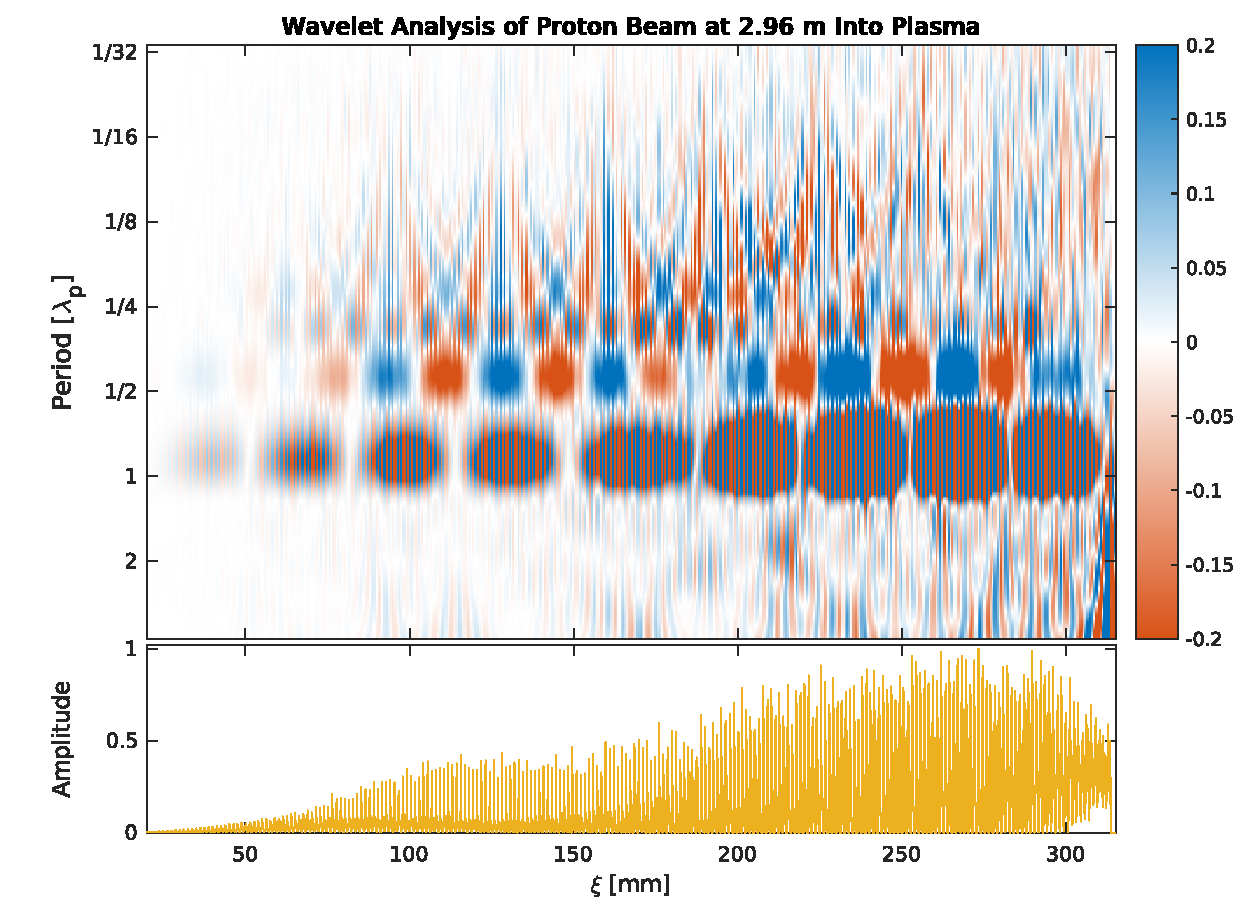
\includegraphics[width=1.0\linewidth]{figures/PBSMIWavelet}
    \caption{\label{Fig:SimA:Wavelet}
        A wavelet analysis of the beam shown in Figure~\ref{Fig:Sim:SMI}, at the same position in the plasma, using a Morlet wavelet \cite{torrence:1998}.
        The horizontal axis shows the position~$\xi$ in the simulation box.
        The vertical axis shows the Fourier period in units of the plasma wavelength~$\lambda_p$.
        This is a density plot of the real component of the transform, showing clearly the peak in frequency in the are around the plasma wavelength.
        The colour axis is cut in order to show the fine structure of the harmonics.
        The higher frequencies are likely dominated by numerical noise.
    }
\end{figure}

% ================================================================================================================================ %
%  Beam Loading and Energy Spread
% ================================================================================================================================ %
\section{Beam Loading and Energy Spread}
\label{SimA:BLoad}

The transverse size of the beam was chosen to be $\sigma_{x,y}=105\unit{\mu m}$, see Table \ref{T:AWAKERuns}.
The longitudinal size was chosen to be $\sigma_{z}=40\unit{\mu m}$ for the studies included in Publication \ref{Pub:IPAC15}, but several lengths were tested in simulations.
$40\unit{\mu m}$ is a good compromise between having a short enough bunch to stay within the accelerating region of the accelerating wakefield, $\approx \lambda_{pe}/4$ (see Section \ref{Int:BPI:BLoad}), and a long enough bunch to contain a reasonable amount of electrons without overloading the wakefield.

% ================================================================================================================================ %
%  Emittance Evolution
% ================================================================================================================================ %
\section{Emittance Evolution}
\label{SimA:Emitt}

Emittance is preserved in the linear regime

% ================================================================================================================================ %
\subsection{The Quasi-Linear Regime}
\label{SimA:QLin}

Text

% ================================================================================================================================ %
\subsection{The Quasi-Linear + Non-Linear Case}
\label{SimA:QLinNonLin}

Quasi-linear reference \cite{rosenzweig:2010}.

An electron beam matched to the typical AWAKE plasma density will be, as discussed in \ref{Int:BPI:Match}, very narrow. At a typical normalised emittance of $2.0\unit{\mu m}$ the beam is $5.25\unit{\mu m}$. Even at low beam charge and at the upper limit in terms of beam length, the wakefields of such a beam will quickly reach the non-linear regime. In the base case used in the beam loading study included in Publication \ref{Pub:BL17} \cite{berglyd_olsen:2018} the peak density of the beam $n_b/n_0 > 35$, well beyond the saturation level of the bubble that occurs when $n_b/n_0 > 10$ \cite{lu:2005}.

The implication here is that there is an additional beneficial effect of loading the accelerating field with as much charge as it will allow without overloading it. The resulting non-linear wake driven by the head of the beam, which will see emittance growth due to the quasi-linear conditions of the proton wake, ensures that the rest of the beam sees a strong focusing force preventing further emittance growth. As the electron beam gains energy, its transverse size will decrease as its emittance is preserved as $\sigma_{r} = \sqrt{\emitN\beta}$ \cite{wille:2001}.

% ================================================================================================================================ %
\subsection{Convergence Scan}
\label{SimA:Converge}

For the large parameter scans performed for Publication~\ref{Pub:BL17}, it was necessary to verify that the results were not dependant on grid resolution.
The radial wakefields within the plasma bubble are linear, but so are the fields within one grid cell as they are interpolated on the grid.
The effect of linear focusing could thus be an artefact of resolution.
Especially in the case where the grid cells were only a factor $2.5$ smaller than the bunch $\sigma_{x,y}$, and thus the bubble radius also small.
\todo[inline]{Verify and cite.}

\begin{table}[hbt]
    \centering
    \caption{Convergence results for a reference simulations for Publication~\ref{Pub:BL17}.
    The reference bunch has a charge of $250\unit{pC}$, and the emittance tolerance criterion for the $\tilde{Q}$ parameter is $5\%$ (see Section~\ref{SimA:QTilde}).}
    \label{T:Converg}
    \begin{tabularx}{132mm}{Xl d{1}l d{1}l d{1}l}
        \rowcolor{tblhead}
        \texthh{Length} & \texthh{Param.}
            & \multicolumn{2}{c}{\texthh{1024$\times$1024}}
            & \multicolumn{2}{c}{\texthh{2048$\times$2048}}
            & \multicolumn{2}{c}{\texthh{4096$\times$4096}} \\
        \hline
                         & $\tilde{Q}$ &  213.9 & $\unit{pC}$  &  206.9 & $\unit{pC}$  &  213.1 & $\unit{pC}$  \\
        $40\unit{\mu m}$ & MEAN$(E)$   & 2263   & $\unit{MeV}$ & 2233   & $\unit{MeV}$ & 2247   & $\unit{MeV}$ \\
                         & STD$(E)$    &  267.4 & $\unit{MeV}$ &  250.4 & $\unit{MeV}$ &  261.5 & $\unit{MeV}$ \\
        \hline
                         & $\tilde{Q}$ &  221.6 & $\unit{pC}$  &  222.0 & $\unit{pC}$  &  222.1 & $\unit{pC}$  \\
        $60\unit{\mu m}$ & MEAN$(E)$   & 2346   & $\unit{MeV}$ & 2336   & $\unit{MeV}$ & 2333   & $\unit{MeV}$ \\
                         & STD$(E)$    &  166.8 & $\unit{MeV}$ &  165.0 & $\unit{MeV}$ &  165.5 & $\unit{MeV}$ \\
        \hline
                         & $\tilde{Q}$ &  229.9 & $\unit{pC}$  &  226.9 & $\unit{pC}$  &  224.8 & $\unit{pC}$  \\
        $80\unit{\mu m}$ & MEAN$(E)$   & 2378   & $\unit{MeV}$ & 2379   & $\unit{MeV}$ & 2368   & $\unit{MeV}$ \\
                         & STD$(E)$    &  120.0 & $\unit{MeV}$ &  117.6 & $\unit{MeV}$ &  119.1 & $\unit{MeV}$ \\
    \end{tabularx}
\end{table}

% ================================================================================================================================ %
\section{Optimising the Witness Beam}
\label{SimA:Opt}

Bringing it all together.

% ================================================================================================================================ %
\section{Summary of Simulation Studies}
\label{SimA:Summary}

\begin{table}[hbt]
    \centering
    \caption{Overview of total simulation cost. $97\%$ of the simulations were run on the supercomputer \textit{Abel}, on Oct Core Intel Xeon E5-2670 CPUs. The remainder were run on older nodes with Quad Core AMD Opteron 2354 CPUs.}
    \label{T:SimCost}
    \begin{tabularx}{\textwidth}{Xlrrr}
        \rowcolor{tblhead}
        \texthh{Topic of Studies}                & \texthh{Code} & \texthh{Count} &     \texthh{CPU Time} &  \texthh{Average} \\
        \hline
        Preliminary studies (mostly testing)     & OSIRIS        &           $21$ &    $266\,599\unit{h}$ & $12\,695\unit{h}$ \\
        Full length AWAKE proton bunch studies   & OSIRIS        &           $38$ &    $440\,583\unit{h}$ & $11\,594\unit{h}$ \\
        Pre-modulated beam studies$^{1}$         & OSIRIS        &          $144$ &    $319\,093\unit{h}$ &  $2\,216\unit{h}$ \\
        3D reference studies                     & OSIRIS        &           $23$ &    $245\,974\unit{h}$ & $10\,695\unit{h}$ \\
        Single drive bunch studies$^{2}$         & OSIRIS        &          $124$ &     $47\,837\unit{h}$ &     $386\unit{h}$ \\
        Beam loading and emittance studies$^{3}$ & QuickPIC      &          $293$ &    $369\,887\unit{h}$ &  $1\,262\unit{h}$ \\
        \hline
        \rowcolor{tblfoot}
        Total                                    &               &          $657$ & $1\,479\,350\unit{h}$ &  $2\,252\unit{h}$ \\
        \multicolumn{5}{p{50mm}}{\footnotesize
            $^{1}$ Main studies for Publication \ref{Pub:IPAC15} \newline
            $^{2}$ Main studies for Publication \ref{Pub:NAPAC16} \newline
            $^{3}$ Main studies for Publication \ref{Pub:BL17} \newline
        }
    \end{tabularx}
\end{table}

% ================================================================================================================================ %

    %
%  Summary and Conclusion
% ========================
%

\chapter{Summary and Conclusion}
\label{Ch:SnC}

Text



% Formatting for Appendices and Publications
\titleformat{\chapter}[display]%
    {\Large\sffamily\scshape}%
    {\textcolor{appendix}\chaptertitlename\ \textcolor{appendix}\thechapter}%
    {2mm}%
    {\Huge\sffamily\upshape}

\addtocontents{toc}{\cftpagenumbersoff{part}}

% Publications

\cleardoublepage
\bookmarksetup{startatroot}
\phantomsection
\part*{Publications}
\label{A:Pub}

\pagestyle{plain}
\renewcommand{\appendixtocname}{Publications}
\renewcommand{\appendixname}{Publication}

\appendix
    \setcounter{chapter}{0}
    \renewcommand{\thechapter}{\Roman{chapter}}
    \renewcommand{\theHchapter}{\Roman{chapter}}
    %
%  Publication 1 :: IPAC 2015
% ============================
%

\chapter{Loading of a Plasma-Wakefield Accelerator Section\\
         Driven by a Self-Modulated Proton Bunch}
\label{Pub:IPAC15}

\begin{hangparas}{10mm}{1}

    \textbf{Abstract:}
    We investigate beam loading of a plasma wake driven by a self-modulated proton beam using particle-in-cell
    simulations for phase III of the AWAKE project. We address the case of injection after the proton beam has already
    experienced self-modulation in a previous plasma. Optimal parameters for the injected electron bunch in terms of
    initial beam energy and beam charge density are investigated and evaluated in terms of witness bunch energy and
    energy spread. An approximate modulated proton beam is emulated in order to reduce computation time in these
    simulations.

    \vspace{8mm}

    \textbf{Authors:}
    Veronica K. Berglyd Olsen, Erik Adli (University of Oslo, Oslo, Norway)
    Patric Muggli (Max Planck Institute for Physics, Munich, Germany)
    Ligia D. Amorim, Jorge M. Vieira (Instituto Superior Technico, Lisbon, Portugal)

    \vspace{5mm}

    \textbf{Publication:}
    Proceedings of IPAC 2015, Richmond, Virginia, USA

    \vspace{5mm}

    \textbf{Date:} 3\ts{rd} to 8\ts{th} of May, 2015

\end{hangparas}

    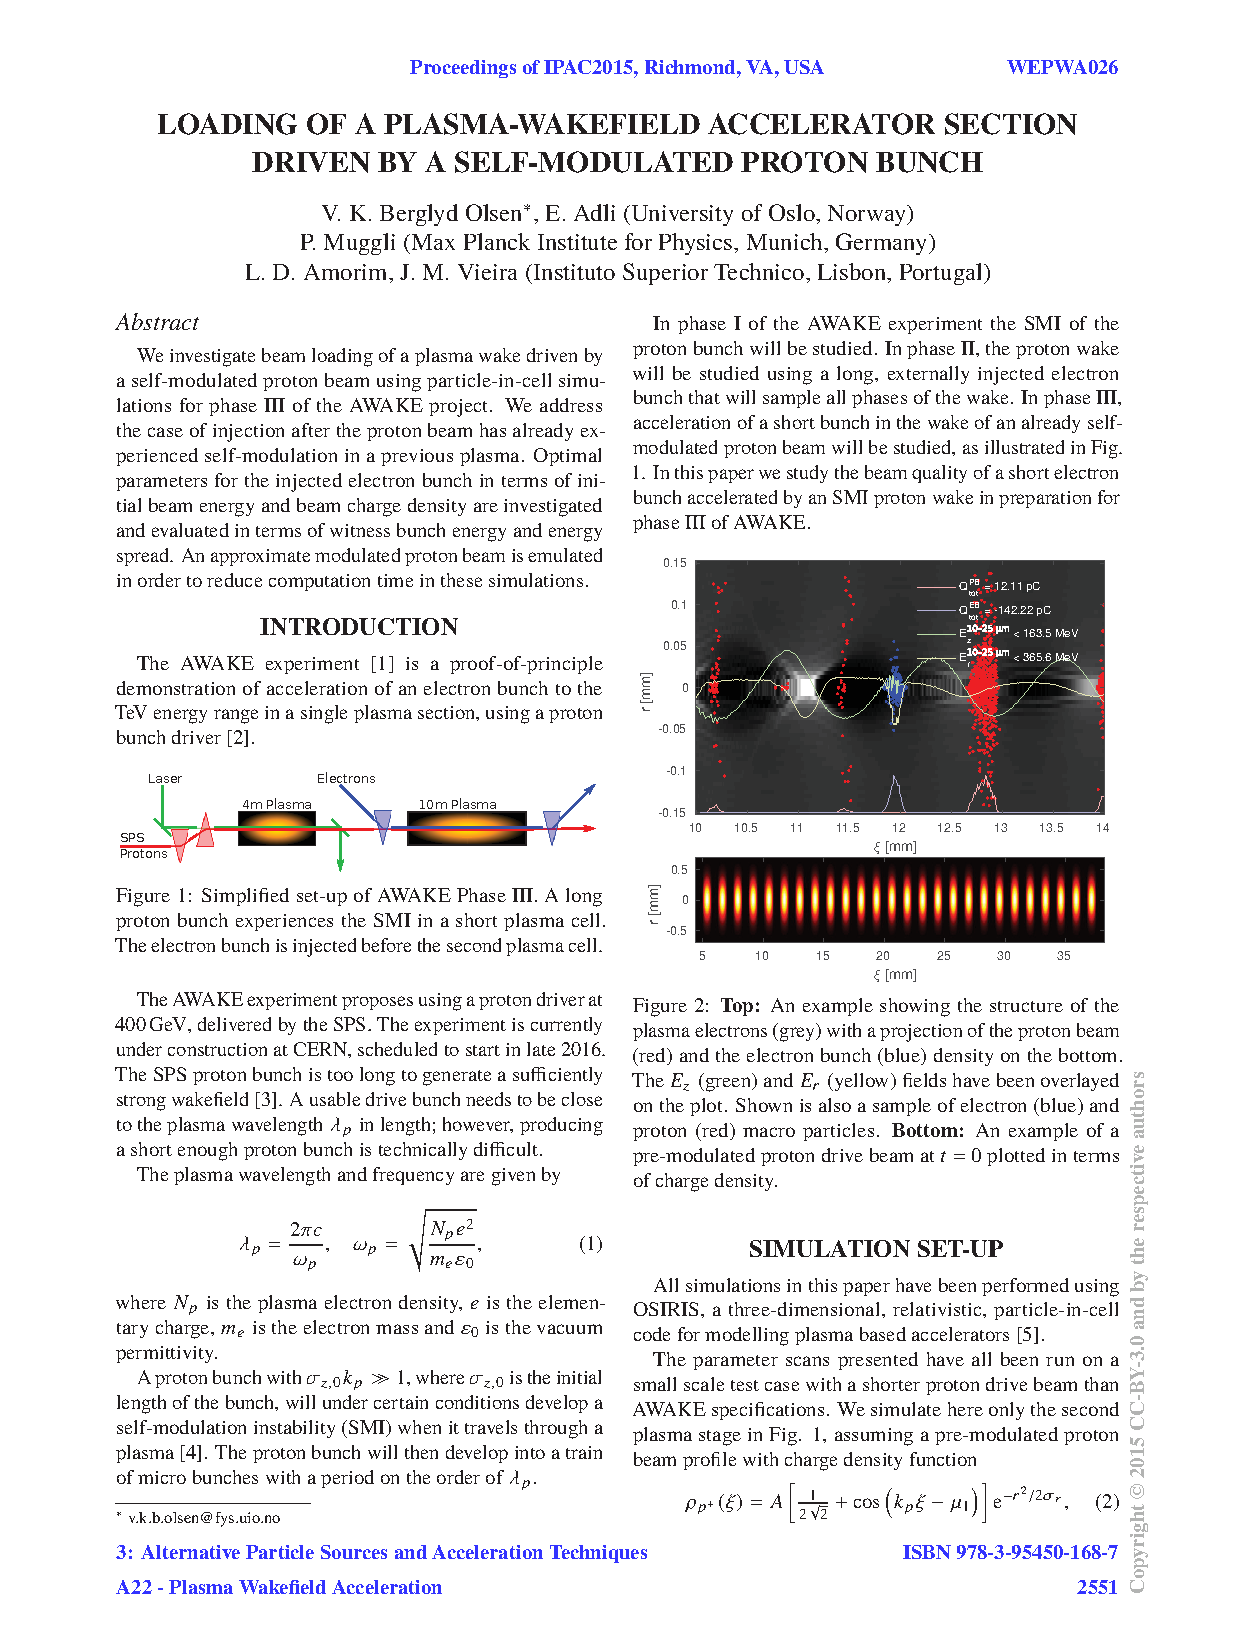
\includepdf[pages=1-last,openright,scale=0.95,pagecommand={}]{files/IPAC15-WEPWA026.pdf}
    %
%  Publication 2 :: NAPAC 2016
% =============================
%

\chapter{Loading of Wakefields in a Plasma Accelerator Section\\
         Driven by a Self-Modulated Proton Beam}
\label{Pub:NAPAC16}

\begin{hangparas}{10mm}{1}

    \textbf{Abstract:}
    Using parameters from the AWAKE project and particle-in-cell simulations we investigate beam loading of a plasma wake driven by a self-modulated proton beam. Addressing the case of injection of an electron witness bunch after the drive beam has already experienced self-modulation in a previous plasma, we optimise witness bunch parameters of size, charge and injection phase to maximise energy gain and minimise relative energy spread and emittance of the accelerated bunch.

    \vspace{5mm}

    \textbf{Authors:}
    Veronica K. Berglyd Olsen, Erik Adli (University of Oslo, Oslo, Norway)
    Patric Muggli (Max Planck Institute for Physics, Munich, Germany and CERN, Geneva, Switzerland)
    Jorge M. Vieira (Instituto Superior Technico, Lisbon, Portugal)

    \vspace{5mm}

    \textbf{Publication:}
    Proceedings of NAPAC 2016, Chicago, Illinois, USA

    \vspace{5mm}

    \textbf{Date:} 9\ts{th} to 14\ts{th} of October, 2016


\end{hangparas}

    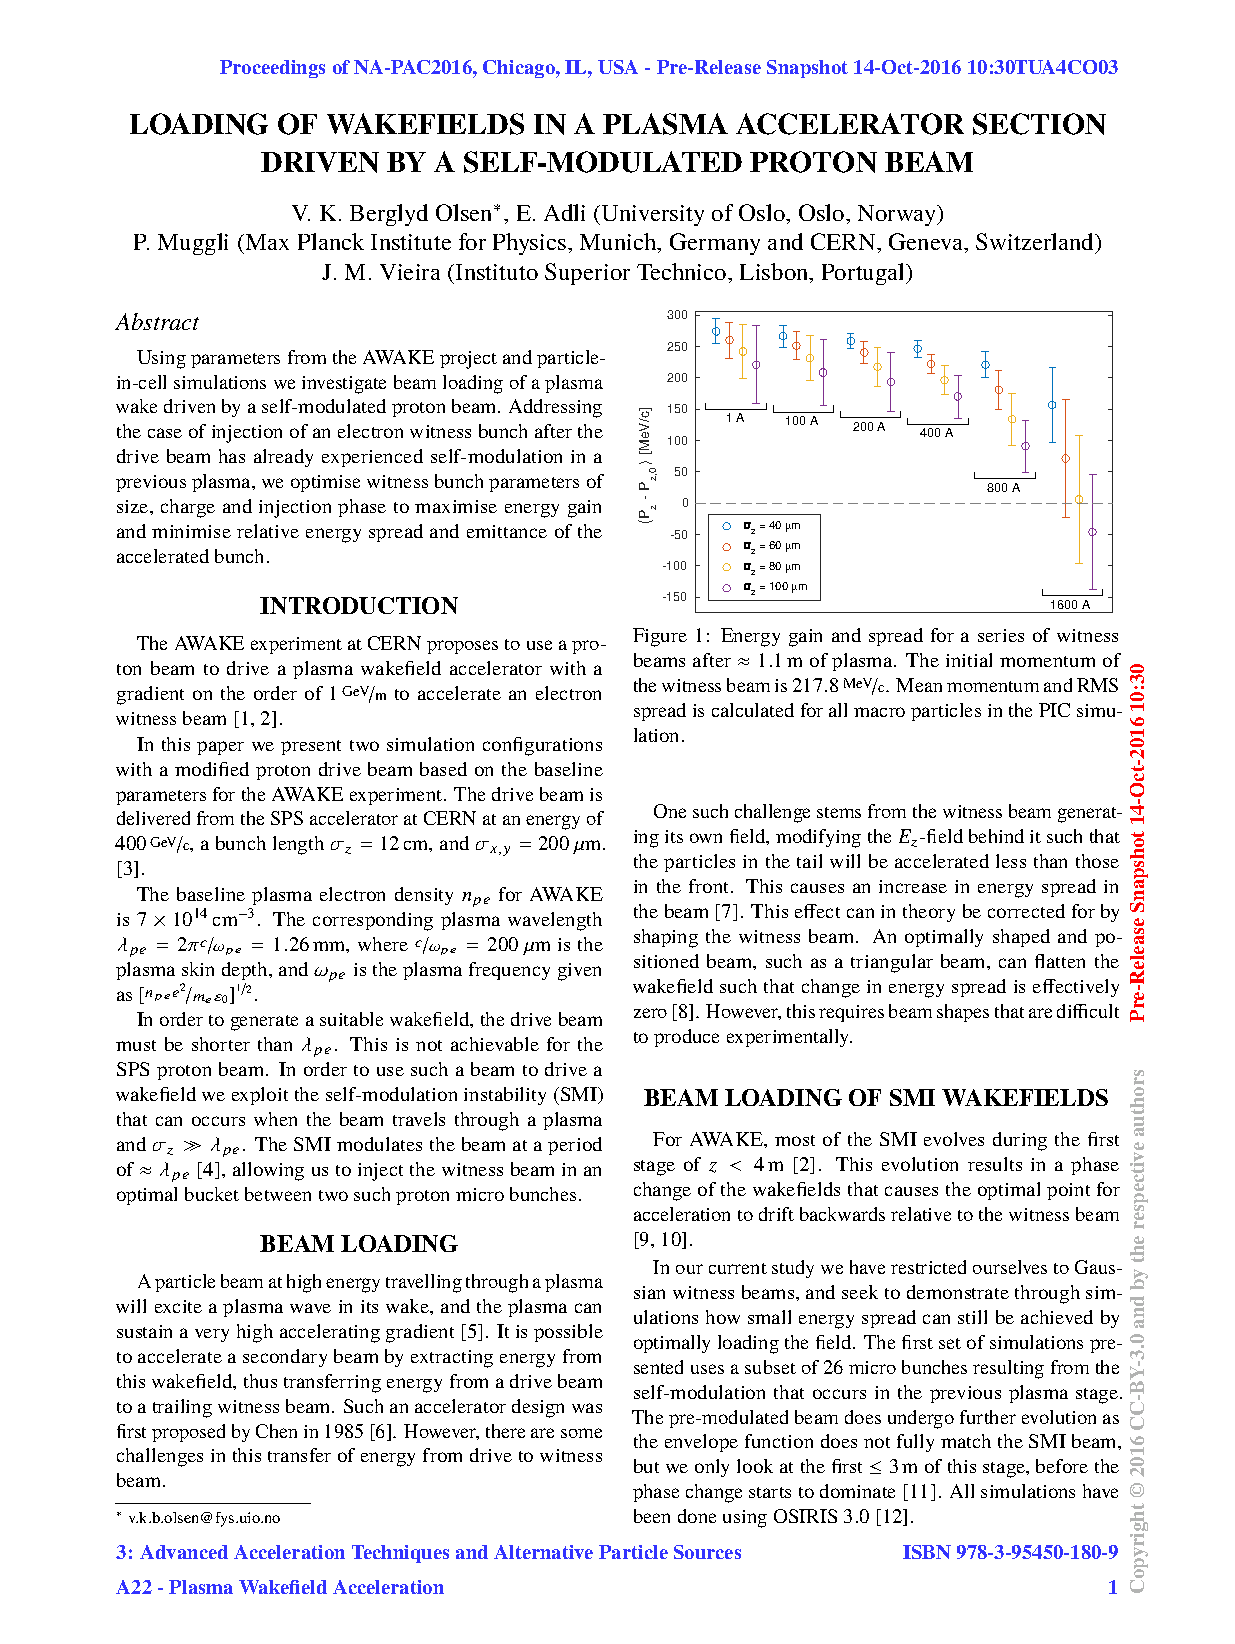
\includepdf[pages=1-last,openright,scale=0.95,pagecommand={}]{files/NAPAC16-TUA4CO03.pdf}
    %
%  Publication 4 :: IPAC 2017
% ============================
%

\chapter{Data Acquisition and Controls Integration of the AWAKE Experiment at CERN}
\label{Pub:IPAC17}

\begin{hangparas}{10mm}{1}

    \textbf{Abstract:}
    The AWAKE experiment has been successfully installed in the CNGS facility at CERN, and is     currently in its first stage of operation. The experiment seeks to demonstrate self-modulation of an SPS proton beam in a rubidium plasma, driving a wakefield of several gigavolt per meter. We describe the data acquisition and controls system of the AWAKE experiment, its integration into the CERN controls system and new control developments specifically required for the AWAKE experiment.

    \vspace{8mm}

    \textbf{Authors:}
    Veronica K. Berglyd Olsen (University of Oslo, Oslo),
    Spencer J. Gessner,
    Jozef J. Batkiewicz,
    Stephane Deghaye,
    Edda Gschwendtner (CERN, Geneva, Switzerland),
    Patric Muggli (Max Planck Institute for Physics, Munich, Germany and CERN, Geneva, Switzerland)

    \vspace{5mm}

    \textbf{Publication:}
    Proceedings of IPAC 2017, Copenhagen, Denmark

    \vspace{5mm}

    \textbf{Date:} 14\ts{th} to 19\ts{th} of May, 2017

\end{hangparas}

    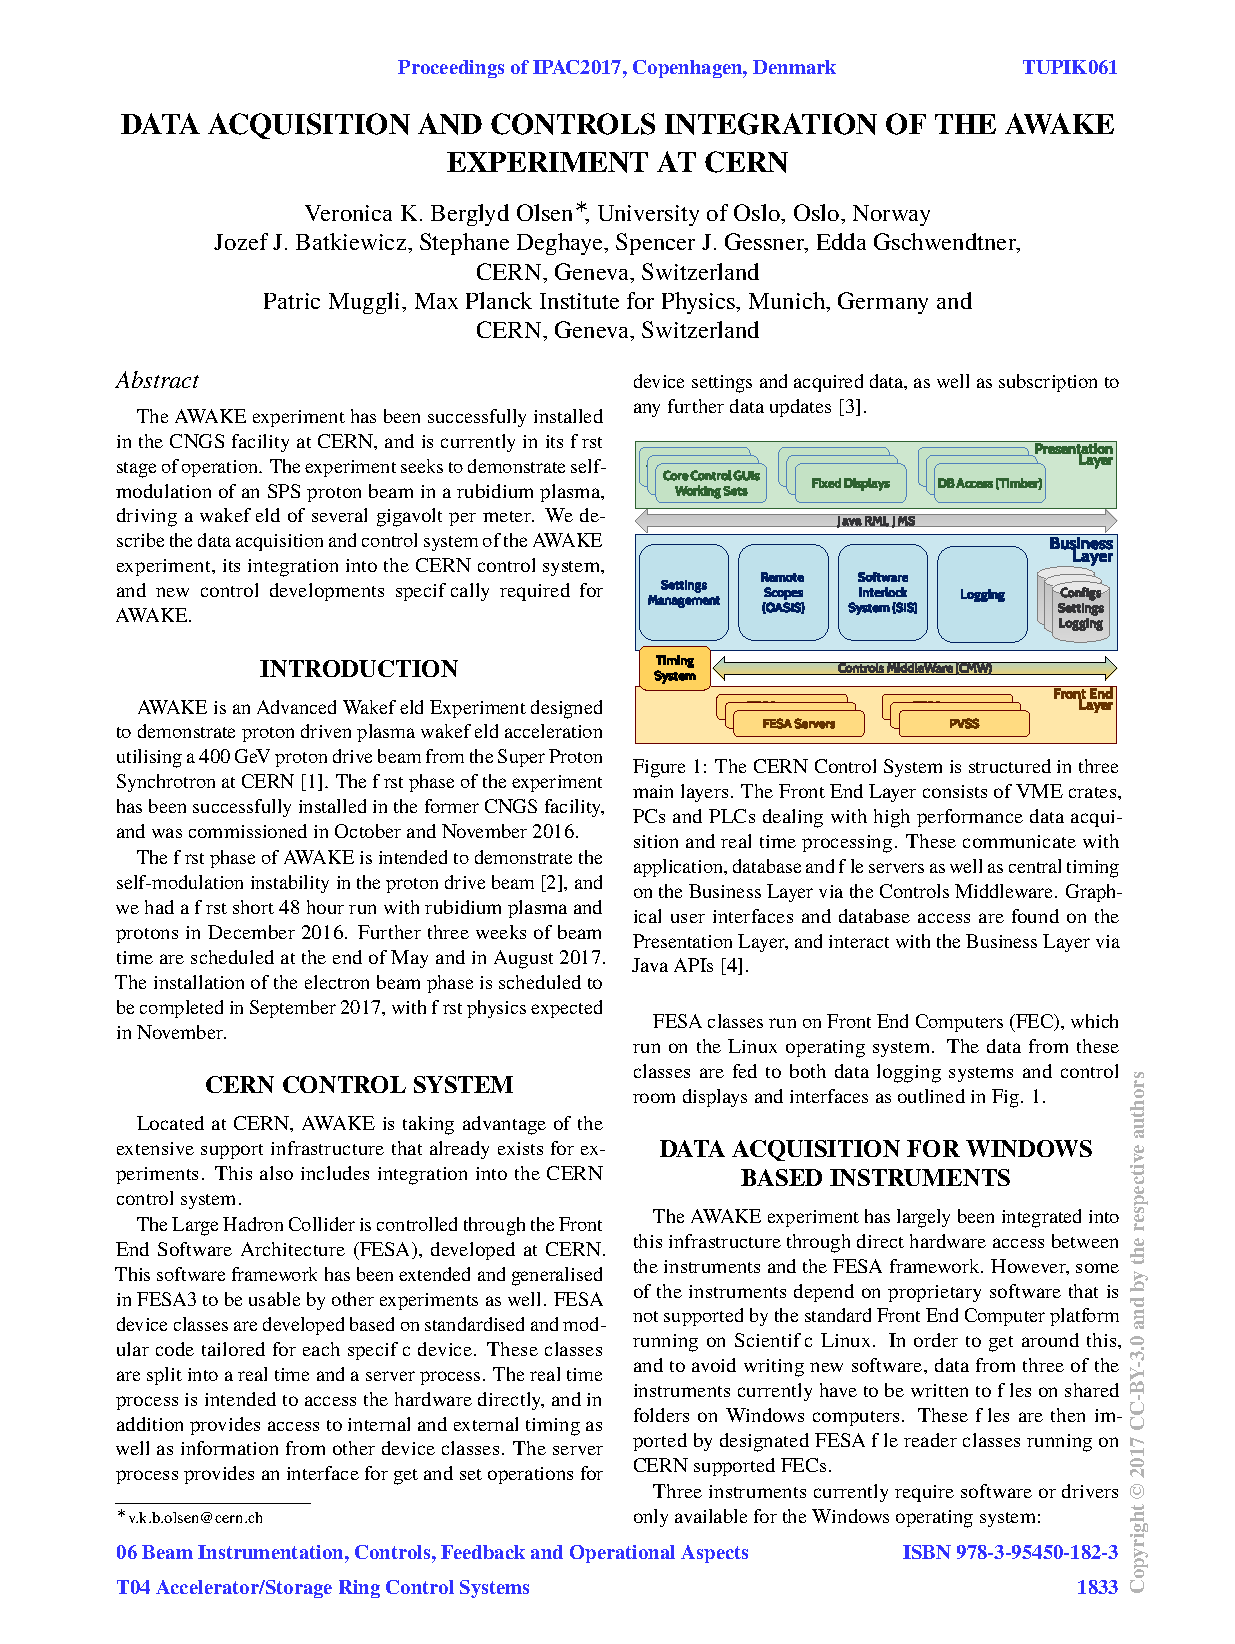
\includepdf[pages=1-last,openright,scale=0.95,pagecommand={}]{files/IPAC17-TUPIK061.pdf}
    %
%  Publication 3 :: Peer Review
% ==============================
%

\chapter{Placeholder Title}
\label{Pub:PRev17}

\begin{hangparas}{10mm}{1}

    \textbf{Abstract:}
    Abstract

    \vspace{8mm}

    \textbf{Authors:}
    Veronica K. Berglyd Olsen (University of Oslo, Oslo)

    \vspace{5mm}

    \textbf{Publication:}
    Journal

    \vspace{5mm}

    \textbf{Date:}

\end{hangparas}

    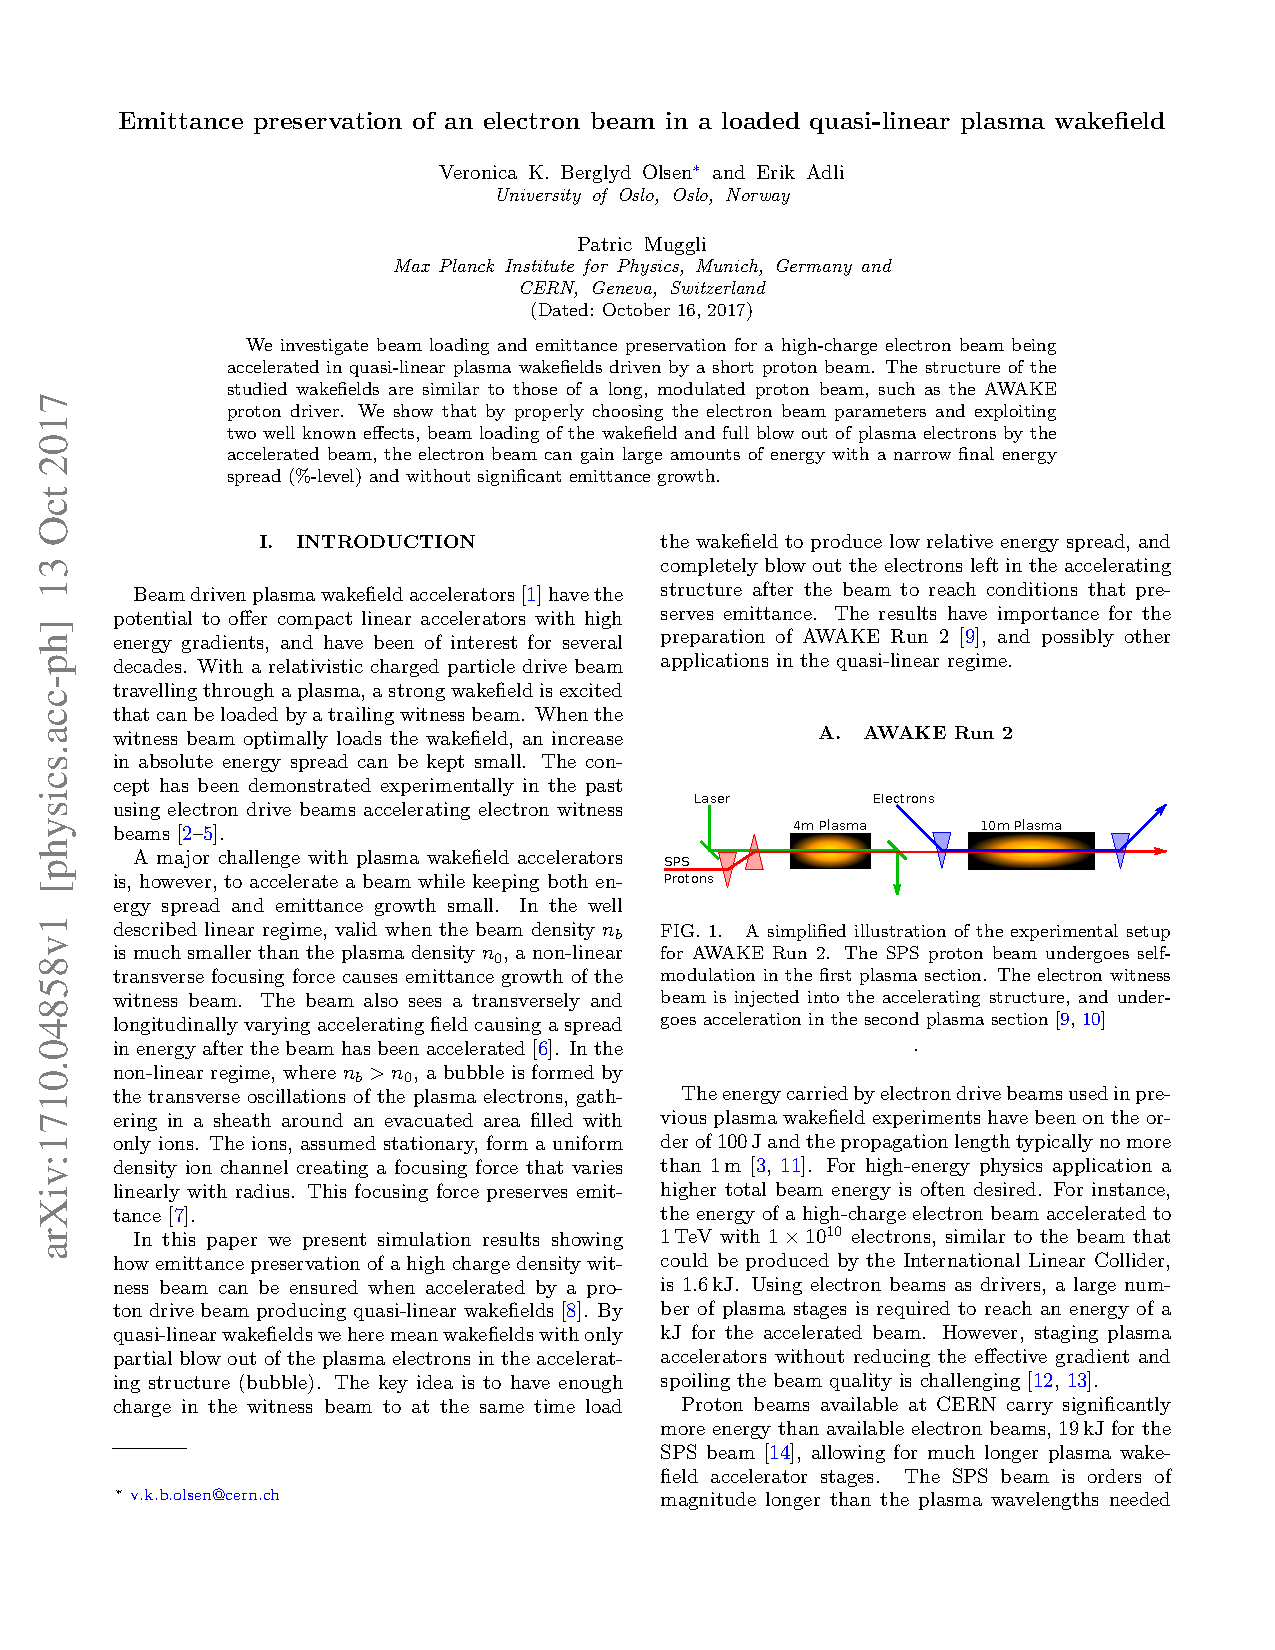
\includepdf[pages=1-last,openright,scale=0.95,pagecommand={}]{files/BeamLoading17.pdf}

% Appendices

\cleardoublepage
\bookmarksetup{startatroot}
\phantomsection
\part*{Appendices}
\label{A:App}

\pagestyle{fancy}
\renewcommand{\appendixtocname}{Appendices}
\renewcommand{\appendixname}{Appendix}
\renewcommand{\headrulewidth}{0.5pt}
\defaulthead

\appendix
    \setcounter{chapter}{0}
    \renewcommand{\thechapter}{\Alph{chapter}}
    \renewcommand{\theHchapter}{\Alph{chapter}}
    %
%  Appendix : PIC
% ================
%

\chapter{Particle in Cell (PIC)}
\label{Apx:PIC}

Some stuff about PIC codes

% ==================================================================================================================== %
\section{Numerical Cherencov}
\label{PIC:NumCher}

    % %
%  Appendix : PIC
% ================
%

\chapter{Data Analysis}
\label{Apx:DA}

The OSIRIS simulation code does not include a data analysis framework. It has been very useful to develop a tool for effective analysis of the large amount of data produced by these simulations.

For the experiment itself a portion of the PhD project has been spent developing data acquistion tools and integrating these with the existing CERN data acquisition infrastructure.

As of the time of writing, the OsirisAnalysis framework is publicly available on GitHub \cite{berglyd_olsen_osirisanalysis:_2013}.

% =============================================================================================== %
\section{Osiris Analysis Framework}
\label{Tools:OA}

The OsirisAnalysis framweork is a modular and object oriented data analysis framweork written in MATLAB. It was designed as a three layer tool to wrap a single data set of OSIRIS simulation data.

\begin{itemize}
    \item \textbf{Layer 1:} Cosnists of the core datawrapper, OsirisData, which provides an interface through which raw data files as well as the simulation input file is parsed. It provides a uniform method for extracting data, and gives access to all the simulation parameters and conversion factors for converting Osiris' normalised units into SI units.
    \item \textbf{Layer 2:} The second layer consists of a set of classes that takes an OsirisData object as input, and returns standardised structs of data that can be scaled and converted to prefered units. They perform often needed tools and methods to parse data and extract more detailed information from the larger raw datasets.
    \item \textbf{Layer 3:} The third layer consist of a number of useful standardised plots and a GUI tool to quickly do a preliminary analysis of simulation data.
\end{itemize}

The philosophy behind this layering of the analysis tool is to allow the user the freedom to choose how many of these they will use. Only using the first layer will give the user access to all the simulation parameters as well as a method to extract data in a standardised manner and return a simple matrix of its content. Adding the second layer gives additional access to automatic unit conversion and other tools if needed. The third layer is entirely optional and simply provides a quick way to browse through the data.

% =============================================================================================== %
\subsection{OsirisAnalysis Core Objects}
\label{Tools:OALay1}

The innermost layer consists of two classes OsirisData and OsirisConfig.

The OsirisData class wraps the simulation data folder and is the core interface through which data is extracted. The class also provides some simple methods for extracting information about the dataset like physical dimensions of the beam and the distribution of the plasma.

The OsirisConfig class is a wrapper for the input file itself, and contains a parser for this file which extracts all the relevant information for both analysis and provides lists of available diagnostics for the graphical user interface (GUI). All conversion factors to SI units are calculated on the fly when the input file is loaded. The OsirisConfig class is not intended to be called by the user, but is found as a child object of the OsirisData data object.

% =============================================================================================== %
\subsection{OsirisAnalysis Data Types}
\label{Tools:OALay2}

The secondary layer of the OsirisAnalysis framework is a set of subclasses under a parent class named OsirisType. The subclasses will give access to specific types of data more or less directly related to the diagnostics types produced by the OSIRIS simulation code.

The classes provided are:

\begin{itemize}
    \item \textbf{Density and Field:} These are classes that produce grid diagnostics data for the particle density data dumps or the field diagnostics data. They support all the different density diagnostics outputs of Osiris, and will in addition calculate the wakefields from the magnetic and electric fields given by $W = F/q = E - v \times B$.
    \item \textbf{Momentum:} The Momentum class consists of a set of methods that will calculate the evolution of the beams energy and momentum over several time dumps.
    \item \textbf{Phase:} The Phase class provides several tools for phase space diagnostics, including calculations of Twiss parameters.
    \item \textbf{UDist:} This class is similar to the Dnesity and Field classes, and provides methods to process velocity and thermal distribution data.
    \item \textbf{Species:} The Species class provides a few additional specialised tools for calculating energy deposition and gain into and from the plasma by the beams, and is also the class where particle tracking data is parsed.
\end{itemize}

In addition to these data parsing classes, there is also a Variables class that will translate Osiris diagnostics variables into readable forms and into strings usable for plot labels. There is also a MathFunc class that provides a math parser that emulates the one used by OSIRIS to parse mathematical functions from the input files. This class is mainly used to extract geometric information about beam density based on the function provided in the input file without the need to first run the code to provide raw particle data.

% =============================================================================================== %
\subsection{OsirisAnalysis Graphical Interface and Plots}
\label{Tools:OALay3}

The final layer of the OsirisAnalysis framwork is a set of very flexible plotting tools. Most of them have a long list of optional input argument. Most of these optional arguments are available through a graphical interface also written in MATLAB named AnalysisGUI.

    %
%  Appendix : Data Analysis Tools
% ================================
%

\chapter{Data Analysis Tools}
\label{Apx:DA}

The simulation codes used in these studies produce large amounts of data.
It has been very useful to develop a tool for effective analysis of both input and output files.
Most of the initial studies were done using OSIRIS 3 (for Publication \ref{Pub:IPAC15} and \ref{Pub:NAPAC16}), and the final emittance study was done using QuickPIC (Publication \ref{Pub:BL17}).

The analysis tools written for these studies are publicly available on GitHub.
The toolbox for OSIRIS 3 is named OsirisAnalysis \cite{code:osiris_analysis:2013}, and the corresponding toolbox for QuickPIC is named QuickPICAnalysis \cite{code:quickpic_analysis:2017}.
Both toolboxes are written for MATLAB.

This appendix briefly outlines the structure and basic function of these tools.

% Also describe briefly how various beam parameters are calculated.
% This should cover Twiss, and the beam quality number used for the last paper.

% ================================================================================================================================ %
\section{The Osiris Analysis Toolbox}
\label{Tools:OA}

The OsirisAnalysis toolbox is a modular and object oriented data analysis toolbox written in MATLAB.
It was designed as a three layer tool to wrap a single data set of OSIRIS simulation data:

\begin{description}
    \item[Layer 1] consists of the core data wrapper class \emph{OsirisData} with its subclass \emph{OsirisConfig}.
        The \emph{OsirisData} class provides an interface for accessing the raw data files, while the \emph{OsirisConfig} class parses the simulation input file.
        \emph{OsirisData} provides a uniform set of calls for extracting the data, and gives through \emph{OsirisConfig} access to all the simulation parameters and conversion factors for converting OSIRS' normalised units into SI units.
    \item[Layer 2] consists of a set of classes that takes an \emph{OsirisData} object as input, and returns standardised structs of data that can be scaled and converted to preferred units.
    They perform often needed tools and methods to parse data and extract more detailed information from the larger raw datasets.
    \item[Layer 3] consist of a number of useful standardised plots, and a GUI tool to quickly do a preliminary analysis of simulation data.
\end{description}

The idea behind this layering of the analysis tool is to allow the user to choose how many of these they will use.
Only using the first layer will give the user access to all the simulation parameters as well as a method to extract data in a standardised manner, and return a simple matrix of its content.
Adding the second layer gives additional access to automatic unit conversion and other data conversion tools like slicing and line-outs, as well as various properties extracted from the macro particle arrays.
The third layer provides a quick way to browse through the datasets and display density plots, phase space plots, Twiss parameters, time evolution, etc.

% ================================================================================================================================ %
\subsection{Core Objects}
\label{Tools:OALay1}

The innermost layer consists of two classes:

\begin{description}
    \item[OsirisData:] This class wraps the simulation data folder and is the core interface through which data is extracted.
    The class also provides some simple methods for extracting information about the dataset like physical dimensions of the beam and the distribution of the plasma.
    
    \item[OsirisConfig:] This class is a wrapper for the input file itself, and contains a parser for this file which extracts all the relevant information for both analysis and provides lists of available diagnostics for the graphical user interface (GUI).
    All conversion factors to SI units are calculated on the fly when the input file is loaded.
    The \emph{OsirisConfig} class is not intended to be called by the user, but is found as a child object of the \emph{OsirisData} data object.
\end{description}

% ================================================================================================================================ %
\subsection{Data Types}
\label{Tools:OALay2}

The secondary layer of the OsirisAnalysis framework is a set of subclasses under a parent class named \emph{OsirisType}.
The subclasses will give access to specific types of data more or less directly related to the diagnostics types produced by the OSIRIS simulation code.

The classes provided are:

\begin{description}
    \item[Density and Field:] These are classes that produce grid diagnostics data for the particle density data dumps or the field diagnostics data.
    They support all the different density diagnostics outputs of OSIRIS, and will in addition calculate the wakefields from the magnetic and electric fields given by $W = F/q = E - v \times B$.
    \item[Momentum:] This class consists of a set of methods that will calculate the evolution of the beams energy and momentum over several time dumps.
    \item[Phase:] This class provides several tools for phase space diagnostics, including calculations of Twiss parameters.
    \item[UDist:] This class is similar to the \emph{Density} and \emph{Field} classes, and provides methods to process velocity and thermal distribution data.
    \item[Species:] This class provides a few additional specialised tools for calculating energy deposition and gain into and from the plasma by the beams, and is also the class where particle tracking data is parsed.
\end{description}

In addition to these data parsing classes, there is also a \emph{Variables} class that will translate OSIRIS diagnostics variables into readable forms, and into strings usable for plot labels.
There is also a \emph{MathFunc} class that provides a math parser that emulates the one used by OSIRIS to parse mathematical functions from the input files.
This class is mainly used to extract geometric information about beam density based on the function provided in the input file without the need to first run the code to provide raw particle data.

% ================================================================================================================================ %
\subsection{Graphical Interface and Plots}
\label{Tools:OALay3}

The final layer of the OsirisAnalysis framework is a set of very flexible plotting tools.
Most of these have a long list of optional input argument that will change the way data is aggregated and presented.
To make these plots easier to use, most of these optional arguments are available through a graphical interface, also written in MATLAB, named \emph{AnalysisGUI}.

\begin{figure}[hbt]
    \centering
    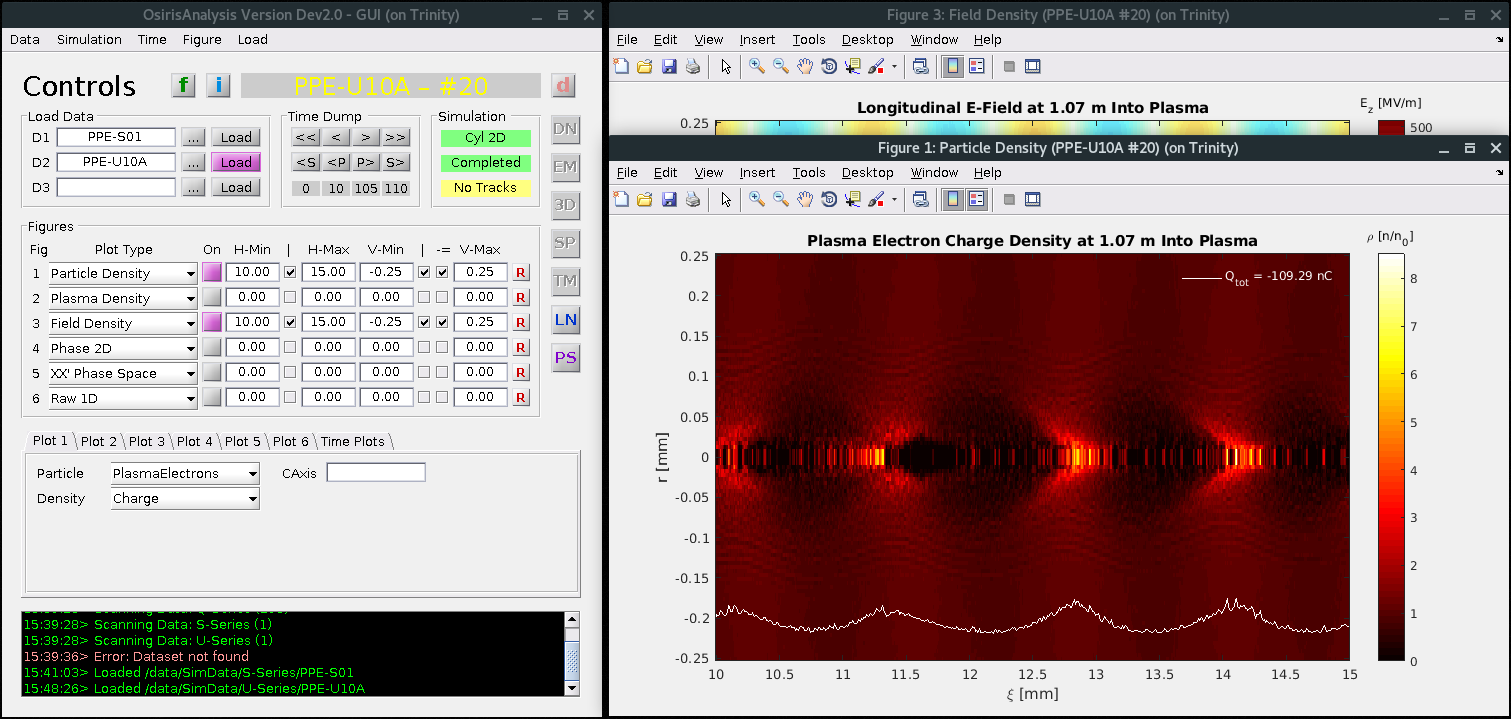
\includegraphics[width=0.99\linewidth,trim={0mm 0mm 0mm 0mm},clip]{images/OsirisAnalysisGUI}
    \caption{\label{Fig:OAGUI} A screenshot of the OsirisAnalysis GUI tool.}
\end{figure}

% ================================================================================================================================ %
\section{QuickPIC Analysis Framework}
\label{Tools:QA}

The toolbox developed for OSIRIS was also partially rewritten to work with QuickPIC simulations.
As QuickPIC uses more or less the same normalised units, the code required little modification to work with these output files.
The conversion was also made easier by QuickPIC having a simpler and more consistent set out output files and formats.

As QuickPIC was only used for the final set of studies, only the core objects and input file wrapper classes, and the data type classes were converted.
No graphical user Interface was developed for this toolbox, and only a few standardised plots were added.
The analysis toolbox is available on GitHub \cite{code:quickpic_analysis:2017}.

% ================================================================================================================================ %
\section{Additional Tools Extending MATLAB Functionality}
\label{Tools:OAAdd}

A number of additional statistics and analysis tools were added due to the lack of MATLAB support, or because alternative methods were beneficial.

\begin{description}
    \item[Weighted Statistics:] Additional functions for weighted mean, percentile and standard deviation used by various parts of both analysis tools were added.
    \item[Weighted Covariance:] The MATLAB \texttt{cov} function does support weighted datasets, but for the OsirisAnalysis tool an exponentially weighted covariance function was used instead \cite{pozzi:2012}.
    This was an attempt to reduce effect of noise in the datasets as this method reduces the impact of statistical outliers.
    For the QuickPIC implementation, the regular MATLAB \texttt{cov} method was used.
    \item[Wavelets:] The Wavelet implementation used in OsirisAnalysis is provided by two script acquired from the websites of The Department of Atmospheric and Oceanic Sciences at The University of Colorado Boulder \cite{torrence:1998}.
\end{description}



% Back Matters

\backmatter

% Revert to standard italics for Bibliography
\renewcommand{\emph}[1]{\textit{#1}}

\bookmarksetup{startatroot}
\cleardoublepage
\phantomsection
\addcontentsline{toc}{chapter}{Bibliography}
\bibliography{Bibliography,Additional}
\null

\phantomsection
\bookmarksetup{startatroot}
\pdfbookmark{End}{EndOfDoc}
\vspace*{\fill}
\footnotesize
\noindent Document compiled on \today~at~\currenttime
\newline
\pdftexbanner
\cleardoublepage

\end{document}

% ================================================================================================================================ %
